\documentclass[10pt,a4paper]{article}
% ============================================================
% Atlas / HOLOGY 9.0 HoloDev proposal - shared preamble
% MGM Laboratory design system, ported to LaTeX (tectonic -X)
% ============================================================

\usepackage[a4paper,top=2.1cm,bottom=2.3cm,left=2.15cm,right=2.15cm,headheight=26pt,headsep=16pt,footskip=32pt]{geometry}

% ---------- Fonts ----------
\usepackage{fontspec}
\defaultfontfeatures{Ligatures=TeX}

\setmainfont{Geist}[
  Path = /Users/mitdeveloper/Library/Fonts/,
  Extension = .otf,
  UprightFont = *-Regular,
  BoldFont = *-SemiBold,
  ItalicFont = *-Italic,
  BoldItalicFont = *-SemiBoldItalic,
]
\newfontfamily\geistlight{Geist}[Path=/Users/mitdeveloper/Library/Fonts/,Extension=.otf,UprightFont=*-Light]
\newfontfamily\geistmedium{Geist}[Path=/Users/mitdeveloper/Library/Fonts/,Extension=.otf,UprightFont=*-Medium]
\newfontfamily\geistmono{GeistMono}[
  Path = /Users/mitdeveloper/Library/Fonts/,
  Extension = .otf,
  UprightFont = *-Regular,
  BoldFont = *-SemiBold,
]

\newcommand{\fontpathAssets}{assets/fonts/}
\newfontfamily\bricolage{BricolageGrotesque}[Path=\fontpathAssets,Extension=.ttf,UprightFont=*-Regular]
\newfontfamily\bricolagemed{BricolageGrotesque}[Path=\fontpathAssets,Extension=.ttf,UprightFont=*-Medium]
\newfontfamily\bricolagesb{BricolageGrotesque}[Path=\fontpathAssets,Extension=.ttf,UprightFont=*-SemiBold]
\newfontfamily\bricolagebd{BricolageGrotesque}[Path=\fontpathAssets,Extension=.ttf,UprightFont=*-Bold]
\newfontfamily\bricolagexb{BricolageGrotesque}[Path=\fontpathAssets,Extension=.ttf,UprightFont=*-ExtraBold]

% ---------- Color tokens (DESIGN_SYSTEM.md 2.1) ----------
\usepackage{xcolor}
\definecolor{cbg}{HTML}{FFFFFF}
\definecolor{csurfacemuted}{HTML}{F7F7F5}
\definecolor{csurfaceinverse}{HTML}{0E1116}
\definecolor{cblue}{HTML}{3A6DC5}
\definecolor{cyellow}{HTML}{F7BF33}
\definecolor{cred}{HTML}{F94141}
\definecolor{cgreen}{HTML}{0F8657}
\definecolor{cblue50}{HTML}{ECF1FA}
\definecolor{cyellow50}{HTML}{FEF6E0}
\definecolor{cred50}{HTML}{FEE5E5}
\definecolor{cgreen50}{HTML}{E2F1EA}
\definecolor{cink}{HTML}{0E1116}
\definecolor{cink2}{HTML}{3B4150}
\definecolor{cink3}{HTML}{6B7280}
\definecolor{cink4}{HTML}{9AA1AD}
\definecolor{cline}{HTML}{ECECEA}
\definecolor{clinestrong}{HTML}{D8D8D2}
\color{cink}

% ---------- Core packages ----------
\usepackage{graphicx}
\usepackage{enumitem}
\setlist{itemsep=0.25em, topsep=0.4em, parsep=0pt}
\usepackage[most]{tcolorbox}
\tcbuselibrary{skins,breakable}
\usepackage{titlesec}
\usepackage{fancyhdr}
\usepackage{array}
\usepackage{longtable}
\usepackage{booktabs}
\usepackage{multicol}
\usepackage{eso-pic}
\usepackage[normalem]{ulem}
\usepackage[hidelinks,colorlinks=true,linkcolor=cblue,urlcolor=cblue,citecolor=cblue,breaklinks=true]{hyperref}
\usepackage{microtype}
\usepackage{parskip}
\setlength{\parskip}{0.55em}
\setlength{\parindent}{0pt}

% ---------- Heading styles (type scale, DESIGN_SYSTEM.md 3.2) ----------
% \section{} itself is kept INVISIBLE on the page (zero-height) - it only
% exists to drive \thesection numbering, the running header, and the TOC.
% Real section headings are drawn by \sectionopener, called right after
% each \section[TocTitle]{} with an empty page-title argument. This lets
% the visual heading (eyebrow + big display title + dek + color rule) be
% fully custom while LaTeX's own numbering/TOC machinery stays correct.
\titleformat{\section}{\relax}{}{0pt}{\relax}
\titlespacing*{\section}{0pt}{0.6em}{0pt}

\titleformat{\subsection}
  {\bricolagesb\fontsize{15pt}{19pt}\selectfont\color{cink}}
  {\thesubsection}{0.5em}{}
\titlespacing*{\subsection}{0pt}{1.1em}{0.5em}

\titleformat{\subsubsection}
  {\bricolagesb\fontsize{12.5pt}{16pt}\selectfont\color{cink}}
  {}{0em}{}
\titlespacing*{\subsubsection}{0pt}{0.9em}{0.35em}

% current section accent color, redefined per section via \sectioncolor
\definecolor{ccurrent}{HTML}{3A6DC5}
\newcommand{\sectioncolor}[1]{\definecolor{ccurrent}{named}{#1}}

% ---------- Header / footer ----------
\pagestyle{fancy}
\fancyhf{}
\renewcommand{\headrulewidth}{0.6pt}
\renewcommand{\footrulewidth}{0pt}
\patchcmd{\headrule}{\hrule}{\color{cline}\hrule}{}{}
\fancyhead[L]{\raisebox{-0.1em}{
\includegraphics[height=7.2pt]{assets/atlas-mark.pdf}}\hspace{4pt}{\geistmono\fontsize{7.6pt}{9pt}\selectfont\color{cink3} ATLAS \textbullet\ HOLOGY 9.0 HOLODEV}}
\fancyhead[R]{{\geistmono\fontsize{7.6pt}{9pt}\selectfont\color{cink3} MGM UNJUK DIRI DULU}}
\fancyfoot[C]{{\geistmono\fontsize{8pt}{10pt}\selectfont\color{cink3} \thepage}}
\fancypagestyle{plain}{\fancyhf{}\fancyfoot[C]{{\geistmono\fontsize{8pt}{10pt}\selectfont\color{cink3}\thepage}}\renewcommand{\headrulewidth}{0pt}}

\usepackage{etoolbox}

% ============================================================
% Custom components
% ============================================================

% ---- Eyebrow label (type scale: eyebrow, 12px, 600, uppercase, tracked)
\newcommand{\eyebrow}[2]{{\geistmono\bfseries\fontsize{9pt}{11pt}\selectfont\textcolor{#1}{\MakeUppercase{#2}}}}

% ---- Section opener: eyebrow + big display title + one-line dek, sets the section's leading color
% #1 = brand color name (cblue/cyellow/cred/cgreen)  #2 = eyebrow text  #3 = title  #4 = dek (one sentence)
\newcommand{\sectionopener}[4]{%
  \sectioncolor{#1}%
  \noindent\eyebrow{#1}{#2}\\[0.35em]
  {\bricolagesb\fontsize{25pt}{29pt}\selectfont\color{cink} #3}\\[0.45em]
  {\fontsize{11.5pt}{16pt}\selectfont\color{cink2} #4}
  \vspace{0.9em}
  \noindent\textcolor{#1!35!white}{\rule{\linewidth}{1.1pt}}
  \vspace{1.1em}
}

% ---- atlasframe: browser-chrome mockup around a real screenshot
% #1 = route text shown in the fake URL bar   #2 = image path   #3 = width (fraction of linewidth)
\newcommand{\atlasframe}[3]{%
  \begin{tcolorbox}[
    enhanced, breakable,
    colback=white, colframe=cline,
    boxrule=0.7pt, arc=6pt, top=0pt, bottom=0pt, left=0pt, right=0pt,
    boxsep=0pt,
  ]
    \colorbox{csurfacemuted}{%
      \begin{minipage}{\dimexpr#3\linewidth-20pt}
        \vspace{5pt}
        \textcolor{cred!70!white}{\footnotesize\textbullet}\,\textcolor{cyellow!85!black}{\footnotesize\textbullet}\,\textcolor{cgreen!70!white}{\footnotesize\textbullet}
        \hspace{6pt}{\geistmono\fontsize{7.6pt}{9pt}\selectfont\color{cink3} atlas.creations.ren#1}
        \vspace{5pt}
      \end{minipage}%
    }\\[-0.05em]
    \includegraphics[width=#3\linewidth]{#2}
  \end{tcolorbox}
}

% ---- Caption line under a framed screenshot / diagram
\newcommand{\framecaption}[1]{{\fontsize{9pt}{12pt}\selectfont\color{cink3} #1}\par\vspace{0.6em}}

% ---- Feature card: icon-less, color-accented card for 2-3 up grids
% #1 = accent color  #2 = title   #3 = body text
\newtcolorbox{featurecardbox}[1]{
  enhanced, breakable,
  colback=white, colframe=cline, boxrule=0.8pt, arc=7pt,
  left=11pt, right=11pt, top=9pt, bottom=9pt,
  borderline west={2.6pt}{0pt}{#1},
}
\newcommand{\featurecard}[3]{%
  \begin{featurecardbox}{#1}
    {\bricolagesb\fontsize{11.5pt}{14pt}\selectfont\color{cink} #2}\\[0.25em]
    {\fontsize{9.6pt}{13pt}\selectfont\color{cink2} #3}
  \end{featurecardbox}
}

% ---- Stat card: big number + label, for KPI rows
\newtcolorbox{statcardbox}[1]{
  enhanced, colback=#1!7!white, colframe=#1!30!white, boxrule=0.8pt, arc=7pt,
  left=10pt, right=10pt, top=9pt, bottom=9pt, halign=center,
}
\newcommand{\statcard}[3]{%
  \begin{statcardbox}{#1}
    {\bricolagexb\fontsize{19pt}{21pt}\selectfont\color{#1!65!black} #2}\\[0.15em]
    {\geistmono\fontsize{7.8pt}{10pt}\selectfont\color{cink3}\MakeUppercase{#3}}
  \end{statcardbox}
}

% ---- Quotebreak: inverse dark section (DESIGN_SYSTEM.md 2.2), use at most once per doc
\newtcolorbox{quotebreakbox}{
  enhanced, breakable,
  colback=csurfaceinverse, colframe=csurfaceinverse, arc=8pt,
  left=22pt, right=22pt, top=20pt, bottom=20pt,
}
\newcommand{\quotebreak}[2]{%
  \begin{quotebreakbox}
    {\bricolagesb\fontsize{16pt}{21pt}\selectfont\color{white} #1}\\[0.5em]
    {\fontsize{10pt}{14pt}\selectfont\color{white!70!black} #2}
  \end{quotebreakbox}
}

% ---- Pattern corner accent: places a small pattern PDF at a page corner
% #1 = pattern pdf basename (in assets/patterns/)  #2 = size  #3 = x offset from margin  #4 = y offset from top
\newcommand{\patterncorner}[4]{%
  \AddToShipoutPictureBG*{%
    \AtPageUpperLeft{\put(#3,-#4){\includegraphics[width=#2]{assets/patterns/#1.pdf}}}%
  }%
}

% ---- Callout box (tip / note), single accent color
\newtcolorbox{calloutbox}[1]{
  enhanced, breakable, colback=#1!6!white, colframe=#1!35!white, boxrule=0.8pt, arc=6pt,
  left=12pt, right=12pt, top=9pt, bottom=9pt,
}

% ---- Diagram frame: plain padded box for full-width diagrams (no browser chrome)
\newtcolorbox{diagramboxenv}{
  enhanced, breakable, colback=white, colframe=cline, boxrule=0.8pt, arc=7pt,
  left=14pt, right=14pt, top=12pt, bottom=10pt, halign=center,
}
\newcommand{\diagrambox}[2]{%
  \begin{diagramboxenv}
    \includegraphics[width=#2\linewidth]{#1}
  \end{diagramboxenv}
}

% ---- tabularray-free simple table style (booktabs based)
\newcommand{\tblhead}[1]{{\geistmono\bfseries\fontsize{8pt}{10pt}\selectfont\color{cink3}\MakeUppercase{#1}}}


\begin{document}

\thispagestyle{empty}

\vspace*{0.2cm}
\noindent
\begin{minipage}[t]{0.62\linewidth}
  {\geistmono\fontsize{8.5pt}{11pt}\selectfont\color{cink3}\MakeUppercase{Proposal Babak Penyisihan}}\\[0.15em]
  {\geistmono\fontsize{8.5pt}{11pt}\selectfont\color{cink3}\MakeUppercase{HOLOGY 9.0 \textbullet\ Cabang Lomba HoloDev \textbullet\ Universitas Brawijaya}}
\end{minipage}%
\hfill
\begin{minipage}[t]{0.3\linewidth}
  \raggedleft
  {\geistmono\fontsize{8.5pt}{11pt}\selectfont\color{cink3} 7 September 2026}
\end{minipage}

\vspace{0.55cm}
\noindent\textcolor{cline}{\rule{\linewidth}{0.8pt}}
\vspace{1.1cm}

\noindent
\raisebox{-0.16em}{
\includegraphics[height=34pt]{assets/atlas-mark.pdf}}\hspace{10pt}%
{\bricolagexb\fontsize{52pt}{52pt}\selectfont\color{cink}Atlas}

\vspace{0.55cm}
\noindent{\fontsize{14.5pt}{20pt}\selectfont\color{cink2}\bricolagemed
Satu ruang kerja terintegrasi untuk manajemen proyek, obrolan tim, dan kolaborasi real-time: lahir dari kebutuhan nyata sebuah laboratorium kampus, kini sepenuhnya sumber terbuka dan bebas biaya langganan bagi siapa pun.
}

\vspace{0.75cm}
\noindent
\includegraphics[width=\linewidth]{assets/ai/cover-hero-test.png}

\vspace{0.85cm}
\noindent
\begin{minipage}[t]{0.31\linewidth}
  \eyebrow{cblue}{Tim}\\[0.3em]
  {\fontsize{12.5pt}{16pt}\selectfont\bricolagesb\color{cink} MGM Unjuk Diri Dulu}
\end{minipage}%
\begin{minipage}[t]{0.37\linewidth}
  \eyebrow{cblue}{Ketua Tim}\\[0.3em]
  {\fontsize{10.5pt}{15pt}\selectfont\color{cink} Muhammad Idham Ma'arif}\\
  {\fontsize{9pt}{13pt}\selectfont\color{cink3} NIM 245150300111024}
\end{minipage}%
\begin{minipage}[t]{0.31\linewidth}
  \eyebrow{cblue}{Asal Universitas}\\[0.3em]
  {\fontsize{10.5pt}{15pt}\selectfont\color{cink} Universitas Brawijaya}\\
  {\fontsize{9pt}{13pt}\selectfont\color{cink3} Fakultas Ilmu Komputer}
\end{minipage}

\vspace{0.65cm}
\noindent
\begin{minipage}[t]{0.5\linewidth}
  \eyebrow{cblue}{Anggota Tim}\\[0.3em]
  {\fontsize{10pt}{15pt}\selectfont\color{cink} Syafa Hadyan Rasendriya}\\
  {\fontsize{10pt}{15pt}\selectfont\color{cink} Nurul Inayah}
\end{minipage}%
\begin{minipage}[t]{0.5\linewidth}
  \eyebrow{cgreen}{Subtema}\\[0.3em]
  {\fontsize{10pt}{15pt}\selectfont\color{cink} Ekonomi Digital}
\end{minipage}

\vfill
\noindent\textcolor{cline}{\rule{\linewidth}{0.8pt}}\\[0.4em]
\noindent{\geistmono\fontsize{8pt}{11pt}\selectfont\color{cink4} AGPL-3.0 \textbullet\ atlas.creations.ren \textbullet\ Digunakan secara produksi oleh Laboratorium MGM, FILKOM UB}

\clearpage

\thispagestyle{plain}
\eyebrow{cblue}{Isi Proposal}\\[0.3em]
{\bricolagesb\fontsize{20pt}{24pt}\selectfont\color{cink} Daftar Isi}
\vspace{0.3em}
\noindent\textcolor{cline}{\rule{\linewidth}{0.8pt}}
\vspace{0.6em}

\renewcommand{\contentsname}{}
\begin{footnotesize}
\end{footnotesize}
{\fontsize{10.5pt}{18pt}\selectfont
\tableofcontents
}
\clearpage

\clearpage
\section[Abstrak]{}
\sectioncolor{cblue}
\eyebrow{cblue}{Ringkasan}\\[0.3em]
{\bricolagesb\fontsize{19pt}{22pt}\selectfont\color{cink} Abstrak}
\vspace{0.15em}\\
\noindent\textcolor{cblue!35!white}{\rule{\linewidth}{1.1pt}}
\vspace{0.55em}

Laboratorium MGM di Fakultas Ilmu Komputer, Universitas Brawijaya, mempunyai lebih dari 65 anggota yang mempunyai dan mengembangkan berbagai macam proyek. Selama ini, komunikasi dan management hanya mengandalkan spreadsheet atau excel dan pesan WhatsApp maupun Discord. Cara tersebut akan susah scale atau berkembang seiring bertambahnya proyek, dikarenakan kompleksitas yang meningkat. Tim sempat mencoba berlangganan Jira, ClickUp, dan Asana, namun biaya per-pengguna per-bulan tidak wajar untuk skala organisasi yang mempunyai budget minim. Opsi self-hosted seperti Plane juga sudah dicoba, namun tetap terdapat biaya ketika jumlah pengguna melewati batas tertentu, dan tidak menyediakan SSO (SAML/OIDC) dengan paket gratis. Ditambah lagi, hampir semua \textit{project management tools} (PMO) proyek yang dicoba tidak ada yang menyertakan platform komunikasi, sehingga kami tetap harus membayar Slack atau Microsoft Teams secara terpisah untuk berkomunikasi.

\textbf{Atlas} dibuat untuk menyelesaikan persoalan tersebut. Atlas adalah sebuah platform kolaborasi tim yang menyatukan manajemen proyek (PMO, mencakup \textit{kanban board}, \textit{list view}, dan \textit{gantt chart}) dengan sistem komunikasi real-time (RTC), \textit{voice all}, catatan dan whiteboard yang bisa dipakai secara kolaboratif, dalam satu aplikasi yang dapat di-\textit{self-host}, \textit{open source} di bawah lisensi AGPL-3.0, dan tidak punya batasan jumlah pengguna ataupun fitur berbayar. Setiap organisasi cukup menjalankan Atlas di infrastruktur mereka sendiri, mempunyai kendali penuh atas data dari aplikasi, dan tanpa biaya untuk alat manajemen proyek dan alat komunikasi yang terpisah.

\textit{Unique selling points} Atlas dibandingkan hanya prototipe untuk kompetisi HOLOGY adalah statusnya hari ini: aplikasi ini \textbf{sudah berjalan secara produksi} dan digunakan sehari-hari oleh seluruh anggota Laboratorium MGM untuk memanage baik project pribadi maupun project di laboratorium, mulai dari perencanaan, koordinasi tim, hingga komunikasi, bukan sekadar demo yang dibangun untuk perlombaan. Godmode, panel kendali swa-hosting Atlas, memungkinkan admin untu mengatur segala hal yang ada di Atlas (kata sandi, \textit{magic link}, OTP telepon, OAuth, OIDC, SAML), \textit{file storage}, dan tema tampilan tanpa menyentuh kode maupun \textit{env file}.

Atlas mengambil subtema \textbf{Ekonomi Digital} HOLOGY 9.0, Atlas menunjukkan bahwa organisasi Indonesia (laboratorium kampus, komunitas, maupun startup tahap awal) tidak perlu terikat pada langganan perangkat lunak asing yang mahal untuk tetap produktif dan terkoordinasi. Dengan membebaskan biaya operasional yang sebelumnya terserap ke banyak layanan SaaS sekaligus menjaga kedaulatan data di tangan organisasi sendiri, Atlas berkontribusi langsung pada pertumbuhan ekosistem digital yang inklusif, berdaya saing, dan berkelanjutan bagi tim-tim di Indonesia.

\clearpage

\section{Latar Belakang}

Laboratorium MGM di Fakultas Ilmu Komputer, Universitas Brawijaya, adalah tempat lebih dari 65 mahasiswa mengerjakan puluhan proyek internal sekaligus, mulai dari pengembangan layanan internal, riset, hingga dukungan operasional laboratorium. Ketua tim proposal ini sendiri ditugaskan membangun layanan internal laboratorium, dan di situlah masalahnya mulai terasa: tidak ada sistem manajemen proyek (PMO) yang layak, dan spreadsheet Excel sama sekali tidak cukup untuk melacak siapa mengerjakan apa, kapan tenggatnya, dan di tahap mana sebuah proyek berada.

\subsection{Tiga jalan buntu yang sudah dicoba}

\begin{description}
\item[SaaS berbayar (Jira, ClickUp, Asana).] Fungsional dan matang, tetapi harga per-pengguna per-bulan langsung membengkak tidak wajar begitu dikalikan 65+ anggota lintas proyek, anggaran yang tidak realistis untuk laboratorium kampus nirlaba.
\item[Self-hosted terbatas (Plane).] Bisa di-\textit{self-host}, tetapi tetap mengenakan biaya begitu jumlah pengguna melewati ambang tertentu, dan fitur Single Sign-On (SAML/OIDC), yang dibutuhkan agar seluruh anggota bisa masuk dengan akun institusi, terkunci di paket berbayar.
\item[Komunikasi terpisah dari kerja (Slack / Microsoft Teams).] Hampir semua alat manajemen proyek yang dievaluasi tidak menyertakan obrolan tim, sehingga laboratorium harus berlangganan alat komunikasi terpisah, membayar dua kali untuk dua kebutuhan yang sebenarnya saling terkait erat.
\end{description}

\subsection{Keputusan: bangun sendiri, dan bagikan}

Setelah tiga jalan tersebut mentok, tim memutuskan untuk membangun platform sendiri yang menyatukan manajemen proyek dan komunikasi tim dalam satu aplikasi yang benar-benar bisa dimiliki oleh laboratorium: di-\textit{self-host} di infrastruktur sendiri, tanpa batas jumlah pengguna, dan tanpa fitur yang dikunci di balik paket berbayar. Karena masalah ini jelas tidak unik milik Laboratorium MGM saja, setiap komunitas, himpunan mahasiswa, dan startup tahap awal di Indonesia kemungkinan besar menghadapi pilihan yang sama antara membayar mahal atau bekerja dengan alat seadanya, Atlas dilepas sebagai perangkat lunak bersumber terbuka di bawah lisensi AGPL-3.0, gratis untuk siapa pun menjalankan dan memodifikasinya. Sebagai gambaran skala persoalan: laboratorium menaungi \textbf{65+} anggota aktif, telah mencoba dan menolak \textbf{3} kategori alat berbayar, akan menanggung kurang lebih \textbf{dua kali lipat} biaya bila alat manajemen proyek dan komunikasi tetap dibeli terpisah, dan kini menjalankan semuanya dengan biaya lisensi \textbf{Rp0} lewat Atlas.

\clearpage
\section[Tujuan dan Manfaat]{}
\sectionopener{cgreen}{Kenapa Ini Penting}{Tujuan dan Manfaat}{Atlas dirancang untuk satu tujuan sederhana: satu platform, seluruh alur kerja tim, tanpa biaya berlapis.}

\subsection{Tujuan pengembangan}

\begin{enumerate}[leftmargin=1.4em]
  \item Menyatukan manajemen proyek (PMO) dan komunikasi tim (chat, suara) dalam satu aplikasi, sehingga tim tidak perlu berpindah-pindah antara alat yang terpisah.
  \item Menyediakan platform yang dapat di-\textit{self-host} sepenuhnya, tanpa batas jumlah pengguna, proyek, maupun fitur yang dikunci di balik paket berbayar.
  \item Mendukung otentikasi tingkat institusi (SSO SAML/OIDC, OAuth, OTP telepon, tautan ajaib) secara gratis, agar organisasi dengan sistem identitas sendiri tetap bisa mengintegrasikan Atlas tanpa biaya tambahan.
  \item Memberi admin kendali penuh atas konfigurasi instansi (Godmode) tanpa perlu menyentuh kode atau berkas konfigurasi server.
  \item Membuktikan kelayakan solusi melalui pemakaian produksi nyata, bukan sekadar purwarupa kompetisi.
\end{enumerate}

\subsection{Manfaat bagi penerima manfaat}

\noindent
\begin{minipage}[t]{0.485\linewidth}
\featurecard{cgreen}{Laboratorium dan himpunan kampus}{Mengelola puluhan proyek dan puluhan anggota dalam satu ruang kerja, tanpa anggaran langganan SaaS yang biasanya mustahil dipenuhi organisasi mahasiswa nirlaba.}
\end{minipage}\hfill
\begin{minipage}[t]{0.485\linewidth}
\featurecard{cgreen}{Startup dan tim kecil tahap awal}{Mendapatkan perangkat PMO dan komunikasi setara produk berbayar sejak hari pertama, sehingga anggaran terbatas bisa dialihkan ke pengembangan produk inti.}
\end{minipage}

\vspace{0.5em}
\noindent
\begin{minipage}[t]{0.485\linewidth}
\featurecard{cgreen}{Komunitas dan organisasi nirlaba}{Menjalankan koordinasi program dan relawan dengan kendali penuh atas data anggota, tanpa bergantung pada kebijakan atau harga sepihak vendor asing.}
\end{minipage}\hfill
\begin{minipage}[t]{0.485\linewidth}
\featurecard{cgreen}{Ekosistem digital Indonesia}{Menambah alternatif perangkat lunak kolaborasi bersumber terbuka yang dapat dipelajari, dimodifikasi, dan dikontribusikan balik oleh komunitas developer lokal.}
\end{minipage}

\vspace{1.1em}
\begin{quotebreakbox}
{\bricolagesb\fontsize{16pt}{21pt}\selectfont\color{white} Dampak yang paling meyakinkan bukan proyeksi, melainkan yang sudah terjadi.}\\[0.5em]
{\fontsize{10pt}{14pt}\selectfont\color{white!70!black} Sejak dipakai penuh oleh Laboratorium MGM, seluruh koordinasi proyek internal (perencanaan tugas, linimasa, dan komunikasi harian 65+ anggota) berjalan di Atlas, menggantikan kombinasi spreadsheet dan obrolan tersebar yang dipakai sebelumnya, tanpa satu rupiah pun biaya langganan bulanan.}
\end{quotebreakbox}

\clearpage

\section{Fitur Aplikasi}

Tujuh modul yang saling terhubung, semuanya berjalan dalam satu instans Atlas yang sama, bukan produk terpisah yang disatukan secara paksa.

\begin{figure*}[t]
\centering
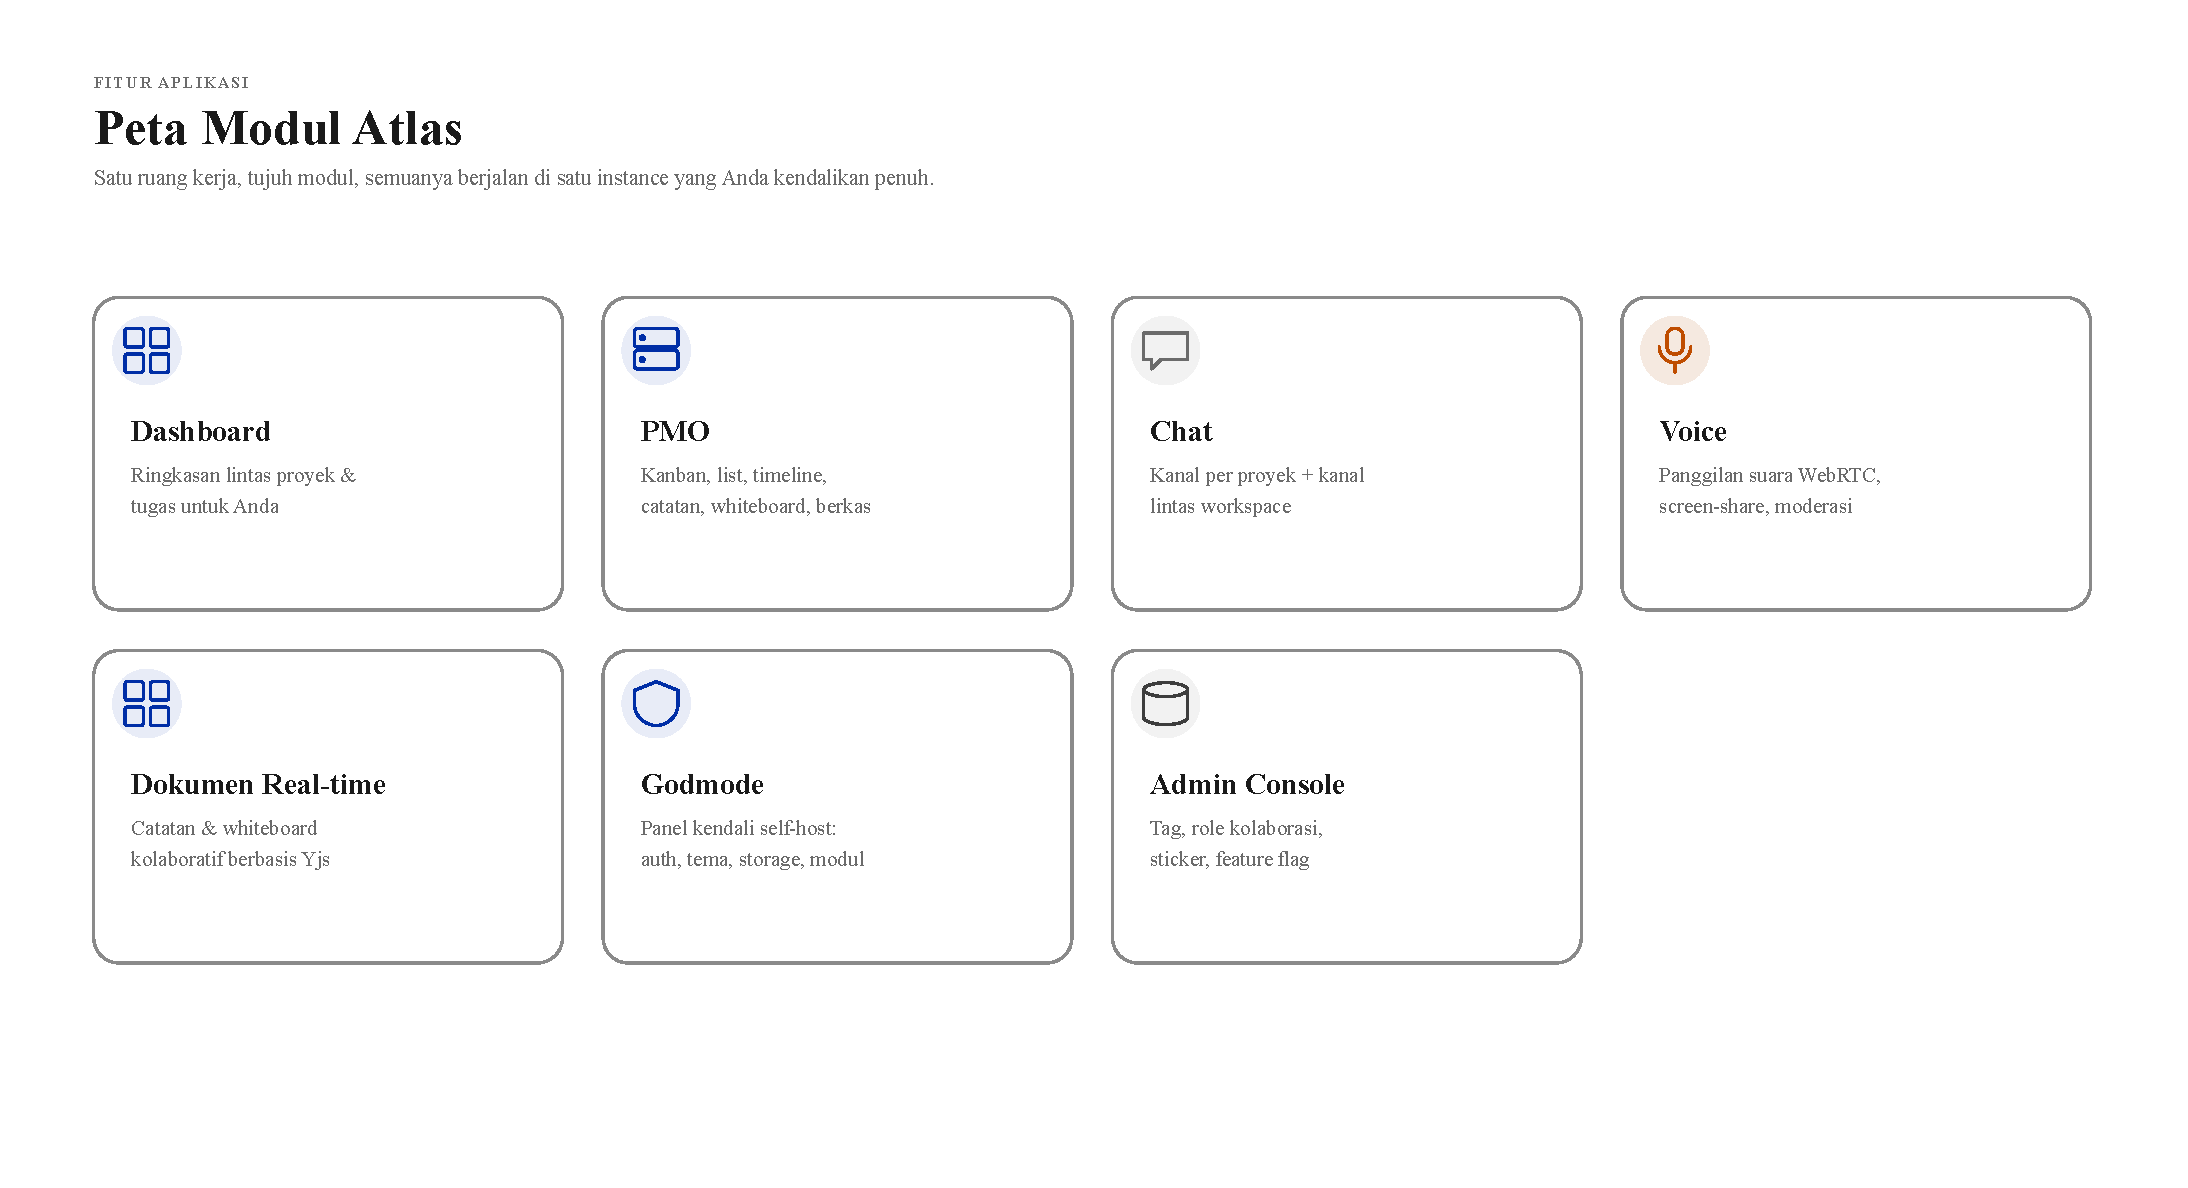
\includegraphics[width=0.72\linewidth]{assets/diagrams/feature-map.pdf}
\caption{Peta fitur Atlas. Setiap modul berbagi identitas pengguna, notifikasi, dan pencarian yang sama.}
\label{fig:feature-map}
\end{figure*}

\subsection{Manajemen Proyek (PMO)}

Setiap proyek memiliki daftar tugas yang bisa ditampilkan sebagai papan Kanban, tabel daftar, atau linimasa Gantt, lengkap dengan status, prioritas, penanggung jawab, dan tenggat waktu. Kunci penomoran tugas (mis.\ \texttt{NO10-14}) tetap unik dan berurutan per proyek meskipun tugas tersebar di banyak daftar berbeda (\cref{fig:pmo}).

\begin{figure*}[t]
\centering
\subfloat[Papan Kanban dengan kolom Backlog, In Progress, In Review, dan Done.]{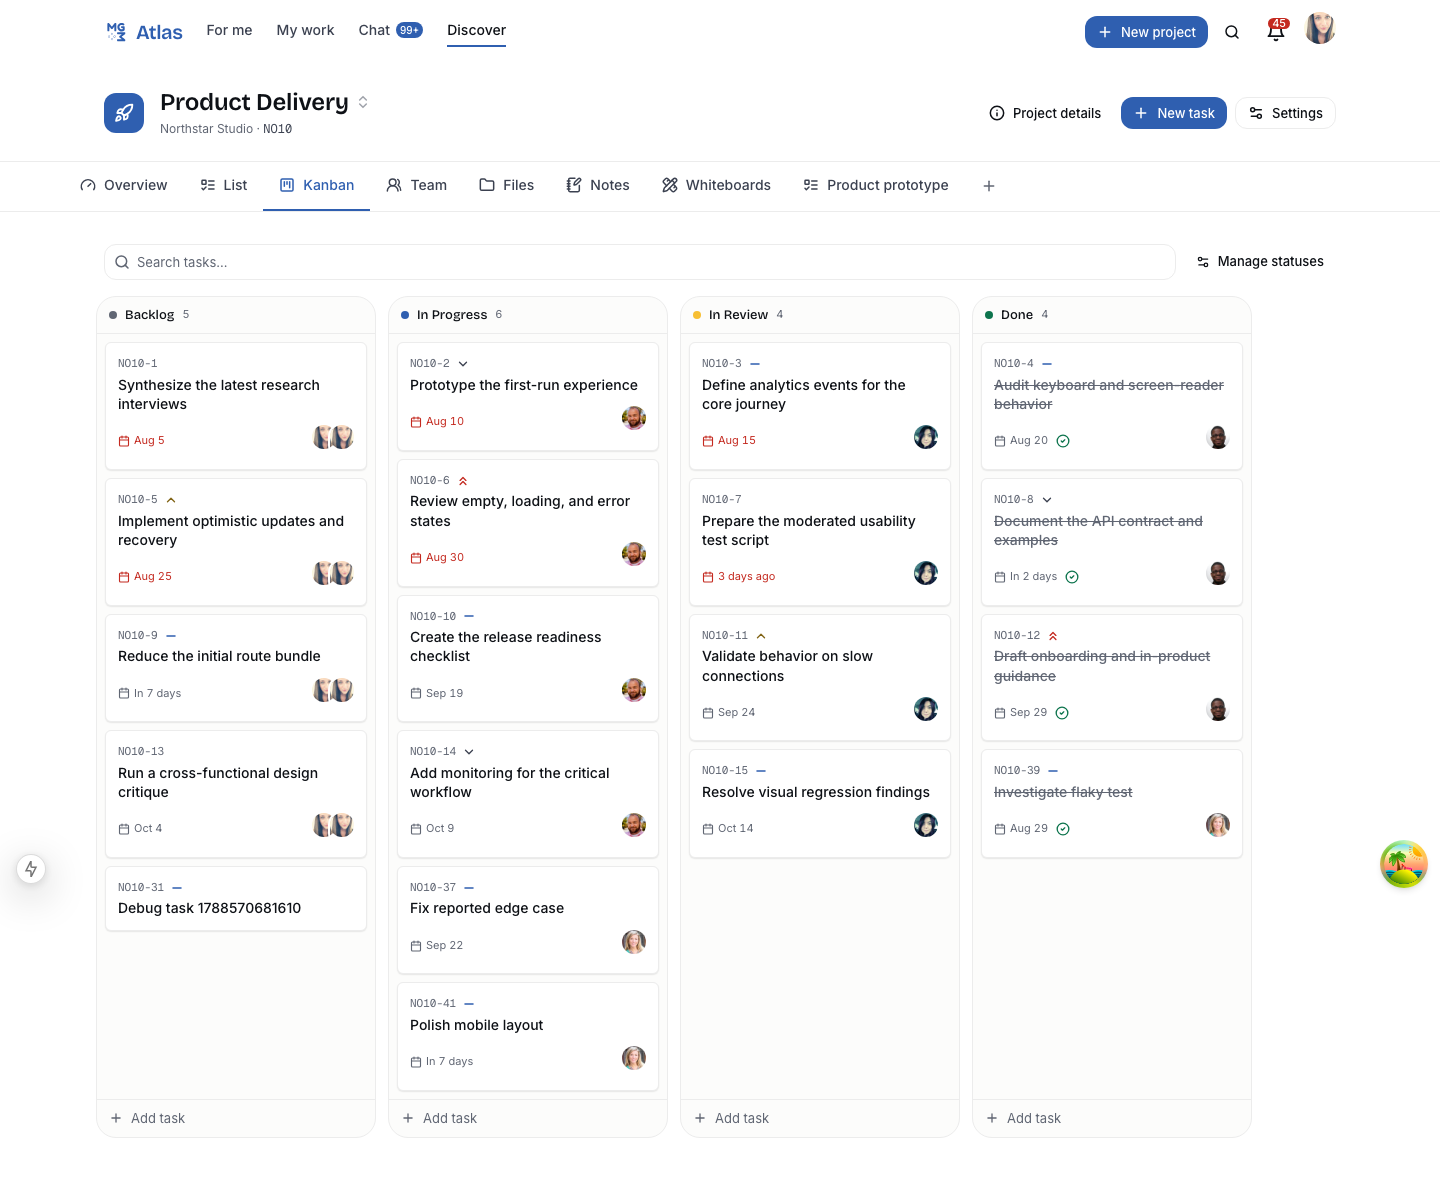
\includegraphics[width=0.485\linewidth]{assets/screenshots/curated/pmo-kanban.png}}\hfill
\subfloat[Detail tugas dibuka sebagai modal di atas papan, tanpa kehilangan konteks.]{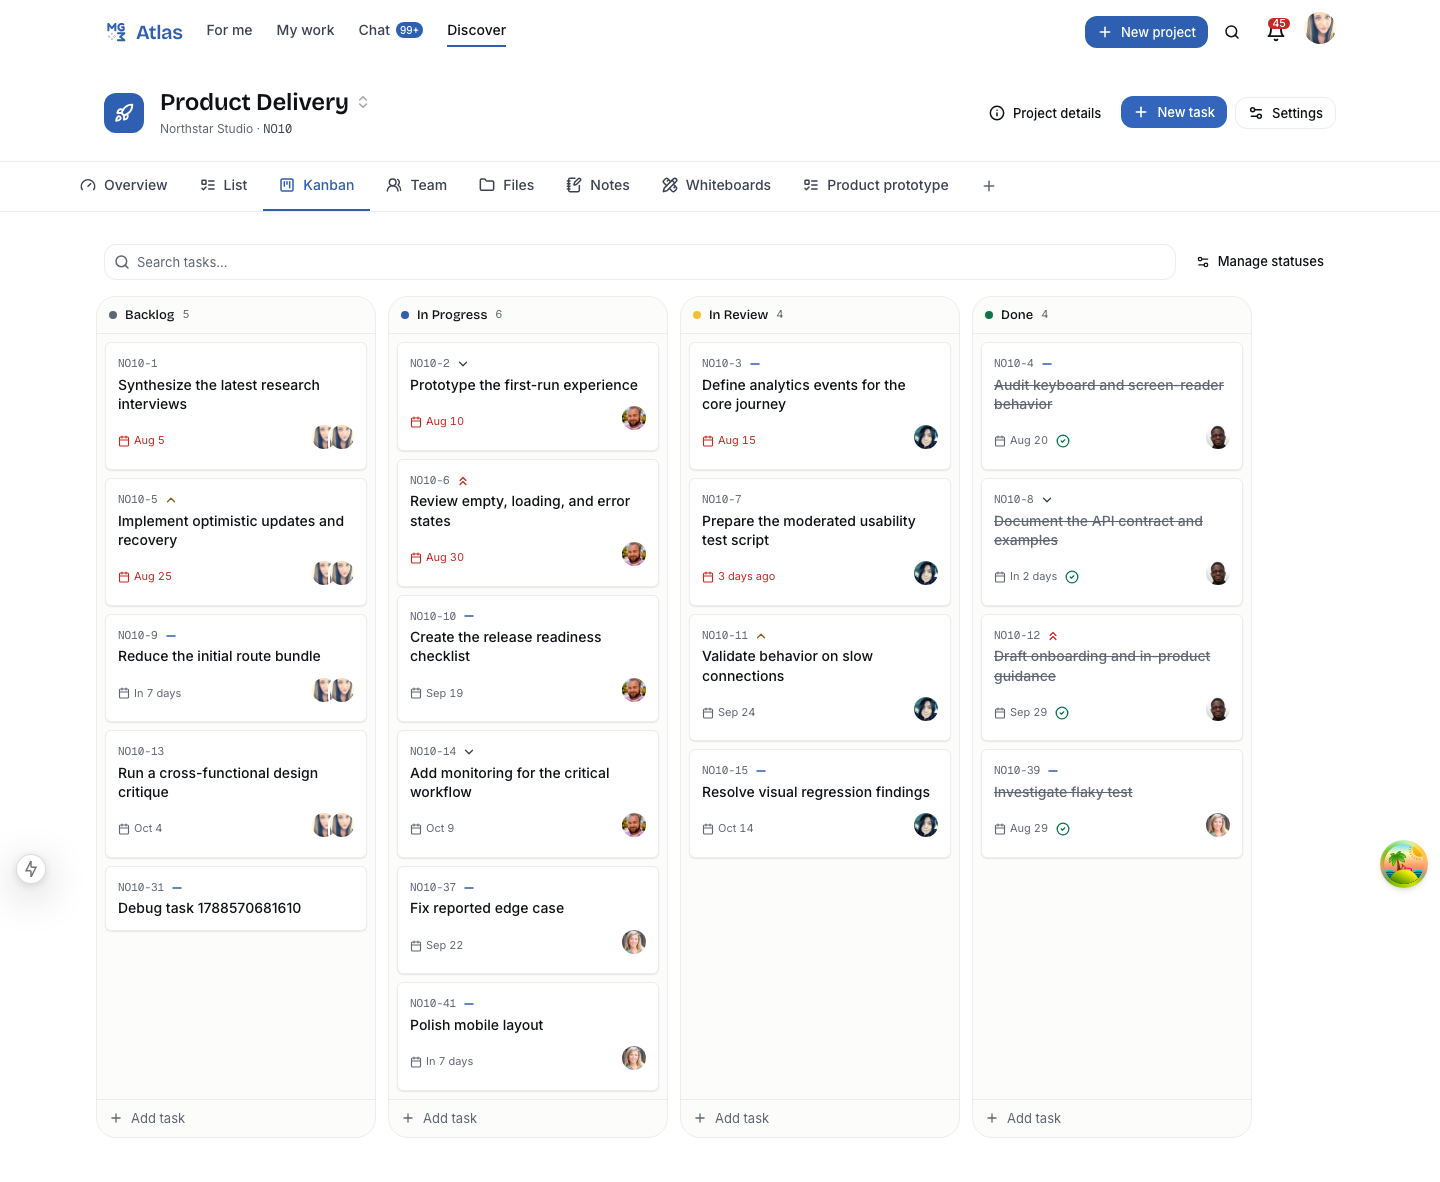
\includegraphics[width=0.485\linewidth]{assets/screenshots/curated/pmo-task-detail.png}}\\[4pt]
\subfloat[Linimasa Gantt untuk melihat jadwal seluruh tugas sekaligus.]{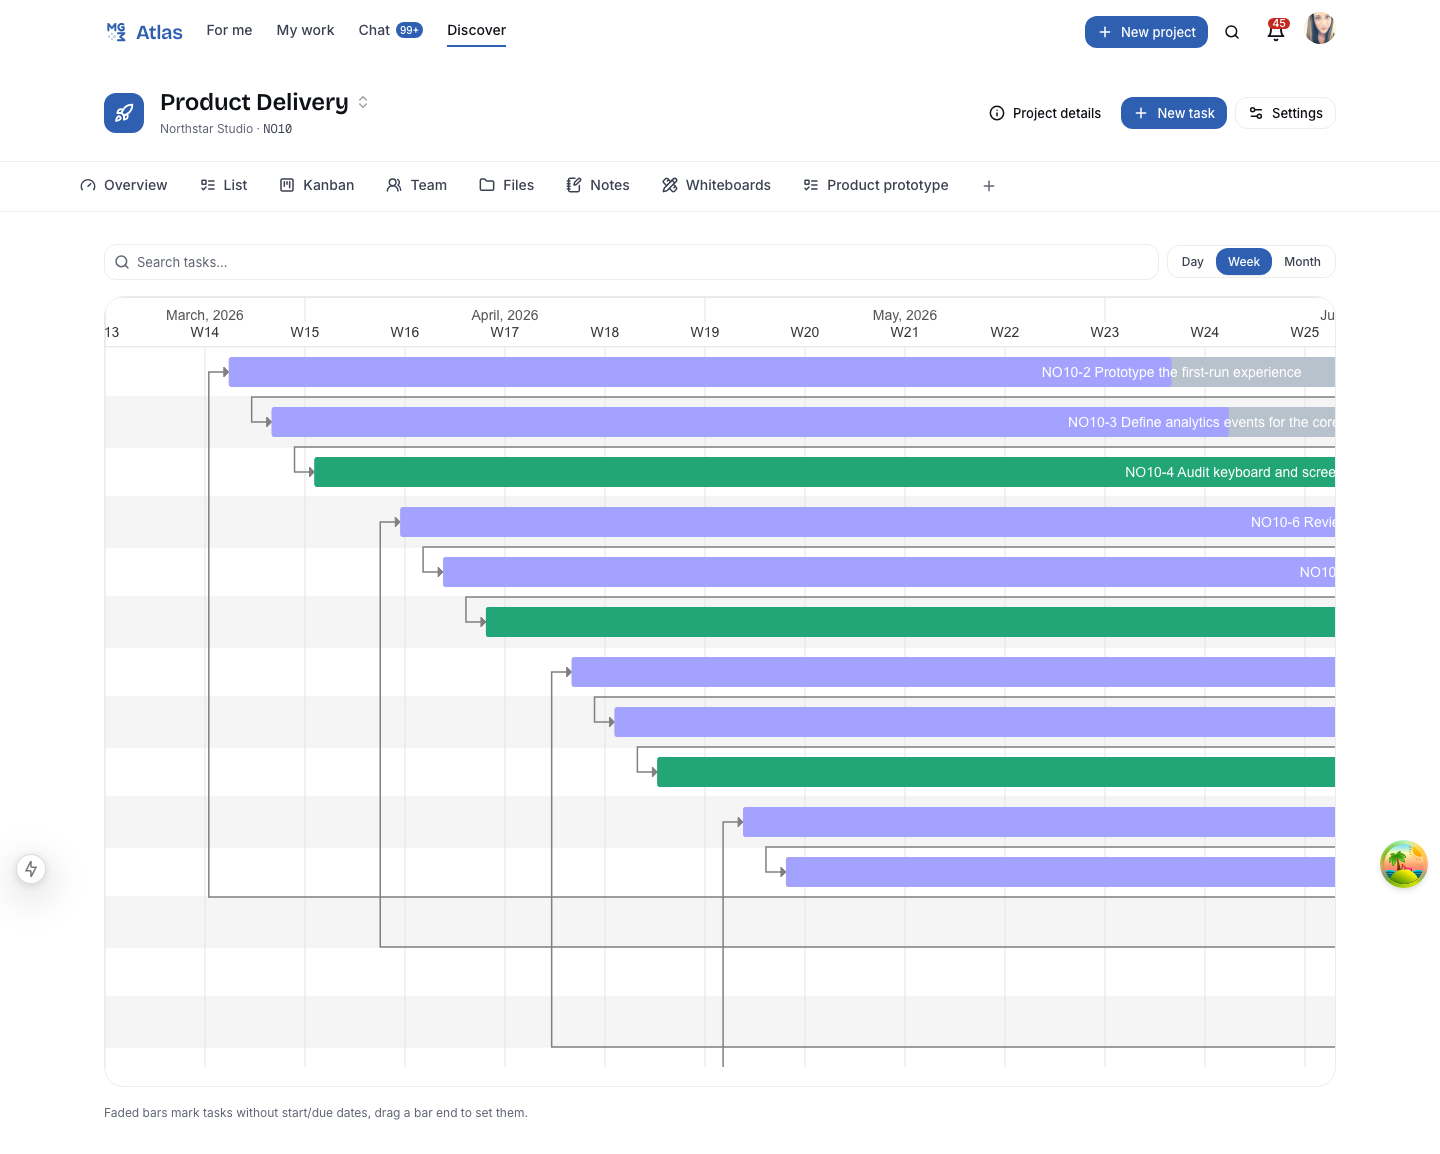
\includegraphics[width=0.485\linewidth]{assets/screenshots/curated/pmo-timeline.png}}\hfill
\subfloat[Whiteboard kolaboratif real-time (Yjs CRDT) untuk pemetaan ide.]{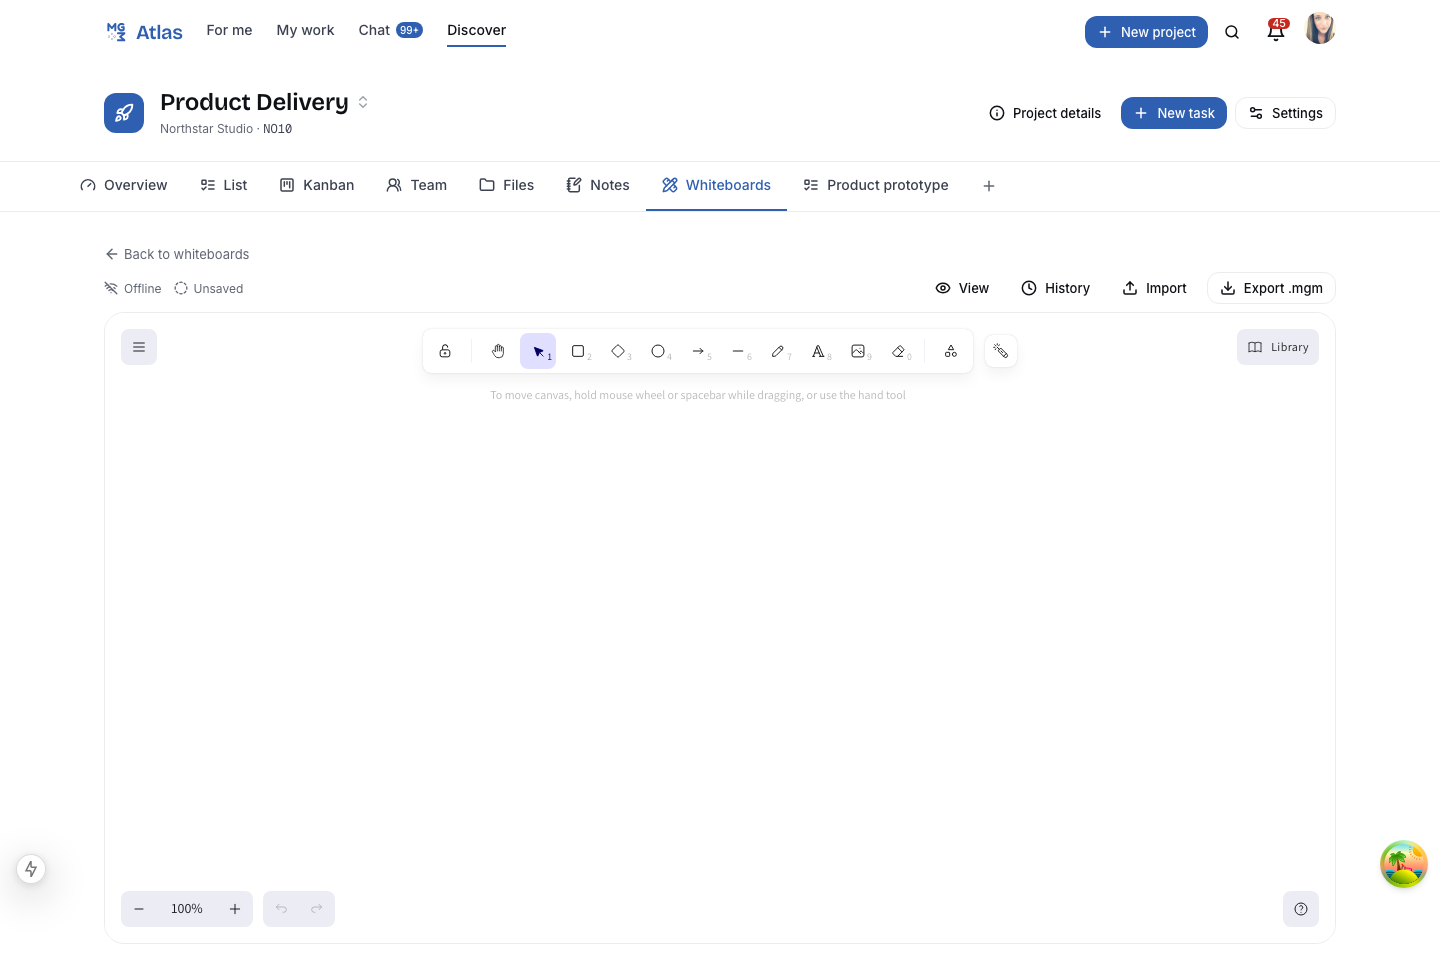
\includegraphics[width=0.485\linewidth]{assets/screenshots/curated/pmo-whiteboard.png}}
\caption{Empat tampilan modul PMO pada proyek yang sama.}
\label{fig:pmo}
\end{figure*}

\subsection{Obrolan Tim dan Panggilan Suara}

Setiap proyek memiliki kanal obrolannya sendiri, ditambah ruang obrolan lintas-tim (\textit{global}) untuk komunikasi seluruh organisasi. Pesan mendukung mention (\texttt{@nama}), reaksi emoji, stiker, lampiran berkas, dan pin. Panggilan suara berjalan lewat LiveKit (WebRTC), langsung antara peserta tanpa melewati server backend sebagai perantara media.

\begin{figure*}[t]
\centering
\subfloat[Obrolan proyek dengan mention, reaksi, dan lampiran.]{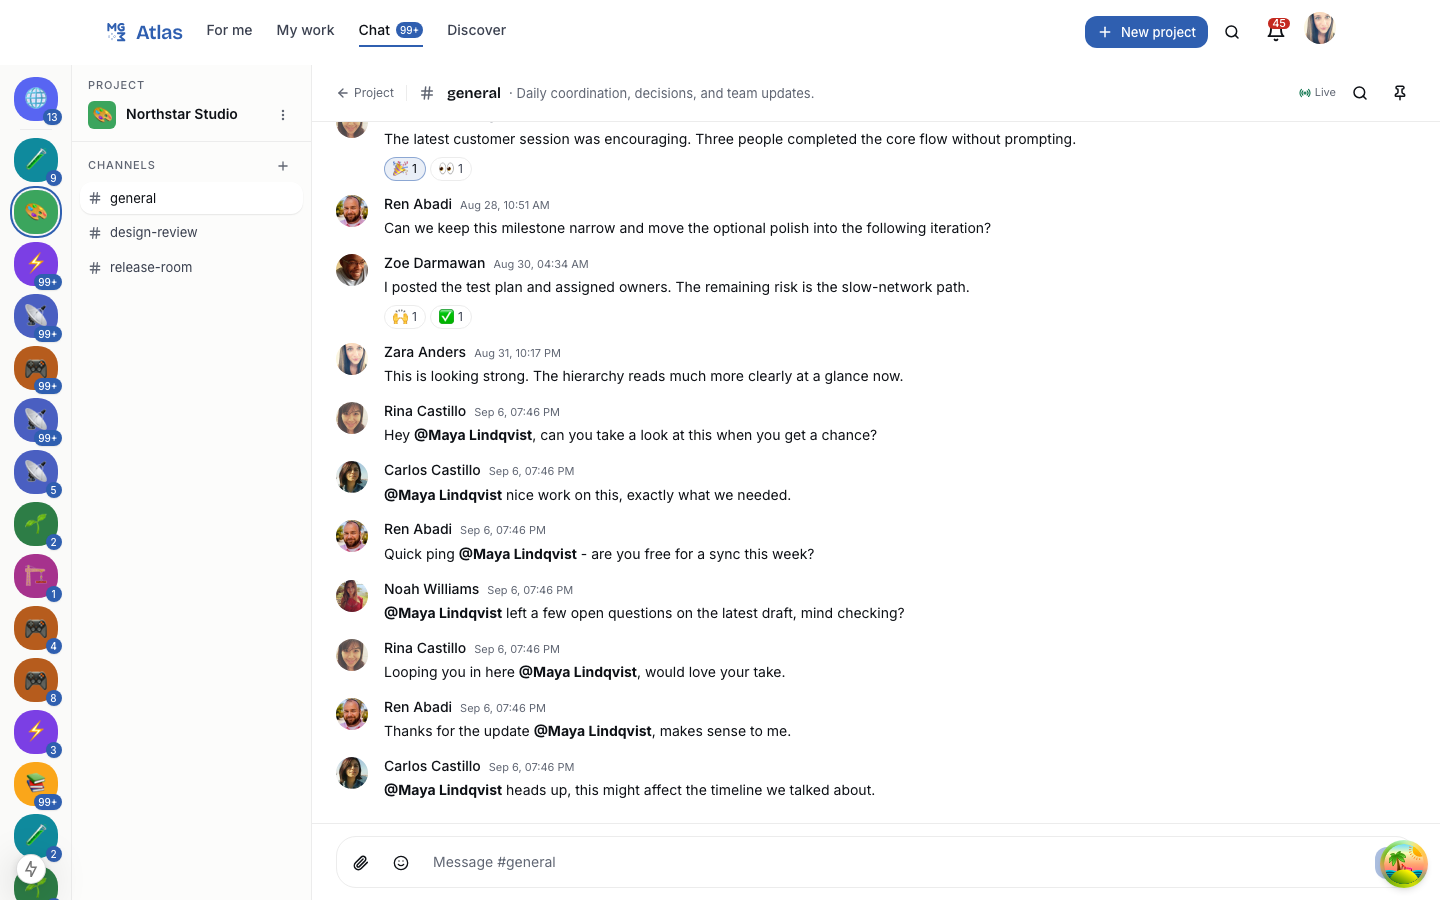
\includegraphics[width=0.485\linewidth]{assets/screenshots/curated/chat-project.png}}\hfill
\subfloat[Ruang suara real-time dengan kontrol mikrofon dan peserta aktif.]{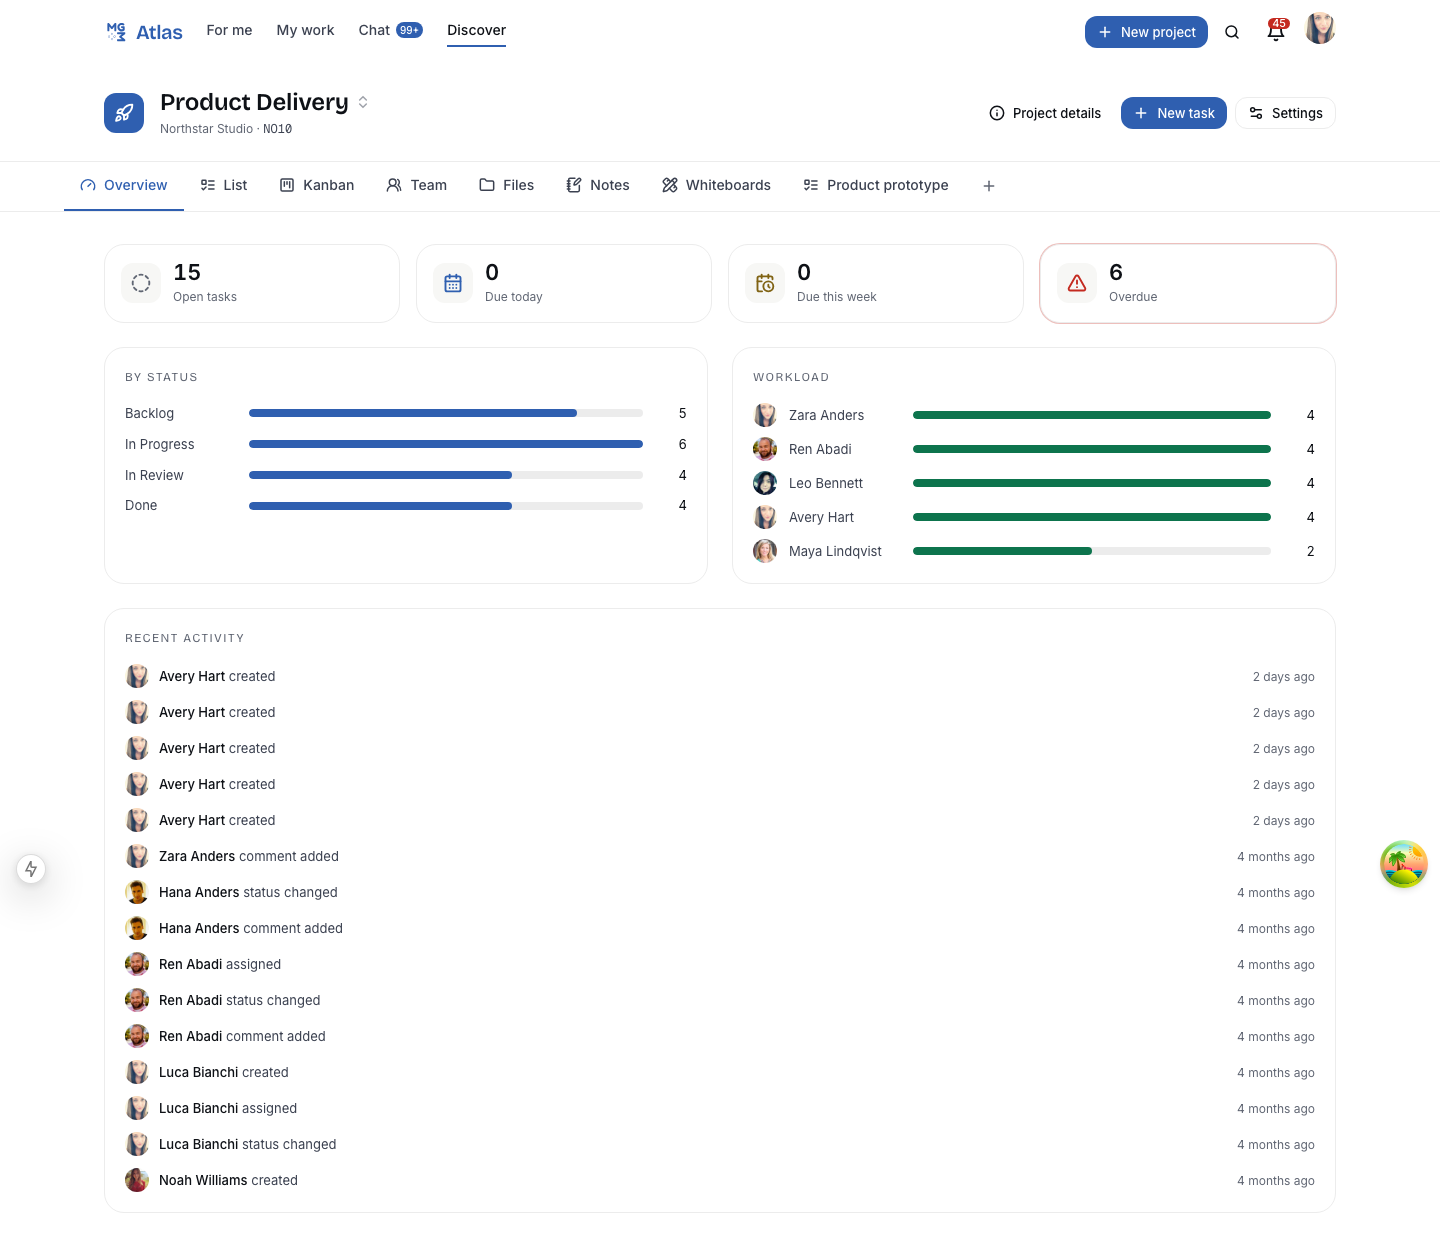
\includegraphics[width=0.485\linewidth]{assets/screenshots/curated/voice-room.png}}
\caption{Komunikasi tim: obrolan dan panggilan suara.}
\label{fig:chat-voice}
\end{figure*}

\subsection{Godmode: Panel Kendali Swa-hosting}

Godmode adalah panel superadmin yang membuat Atlas benar-benar layak dipakai organisasi lain tanpa bantuan developer: metode masuk, penyedia OAuth/SSO, penyimpanan berkas, tema tampilan, dan modul fitur, semuanya diatur lewat antarmuka, bukan berkas \texttt{.env}.

\begin{figure*}[t]
\centering
\subfloat[Ringkasan status instans dan progres konfigurasi awal.]{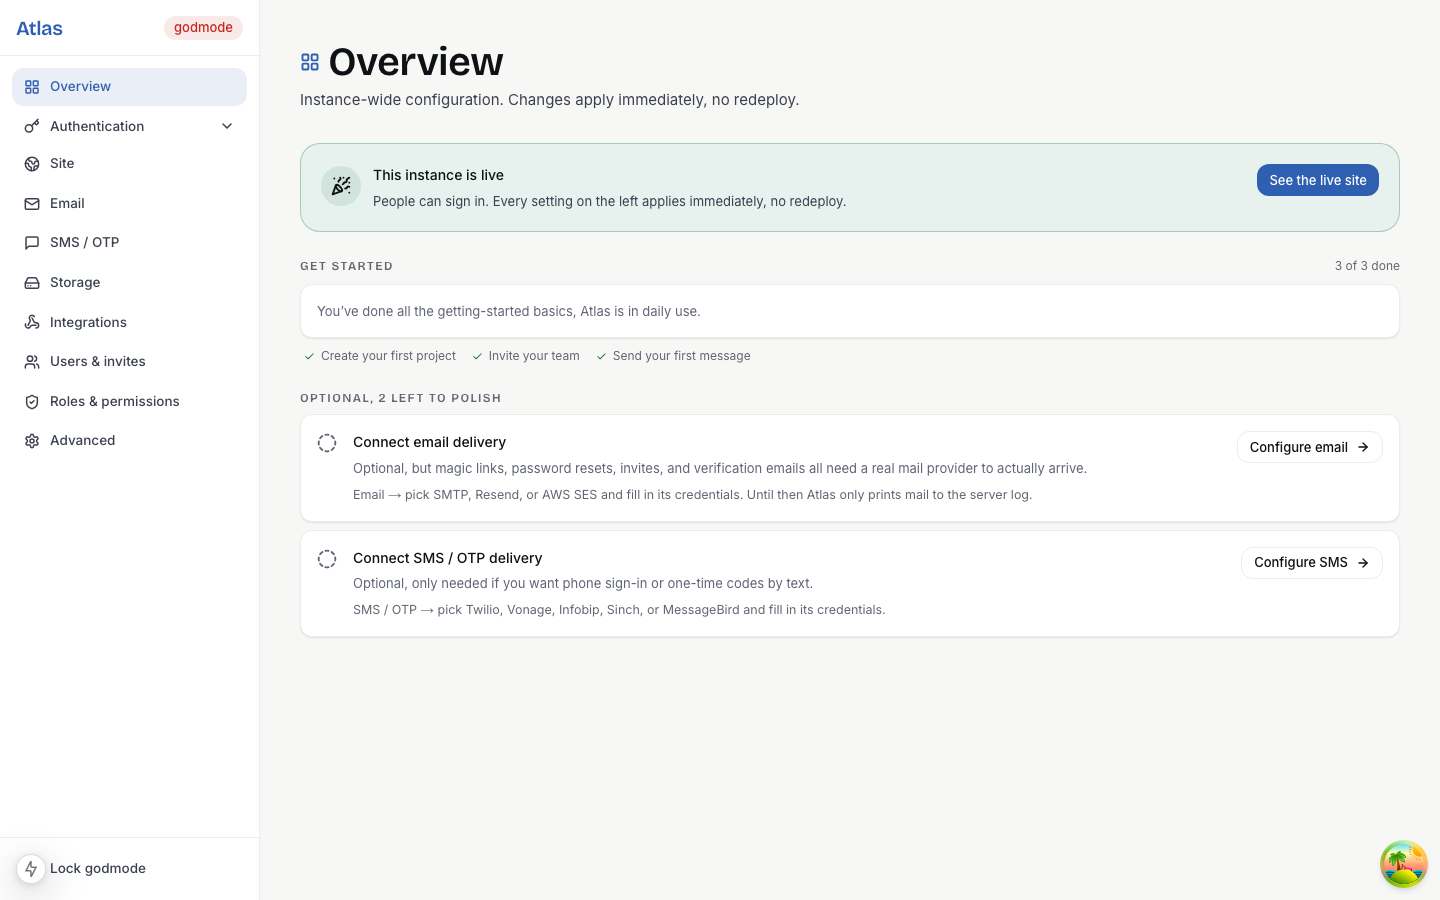
\includegraphics[width=0.485\linewidth]{assets/screenshots/curated/godmode-overview.png}}\hfill
\subfloat[Penyedia OAuth (Google, GitHub, Discord, dan lainnya) diaktifkan tanpa deploy ulang.]{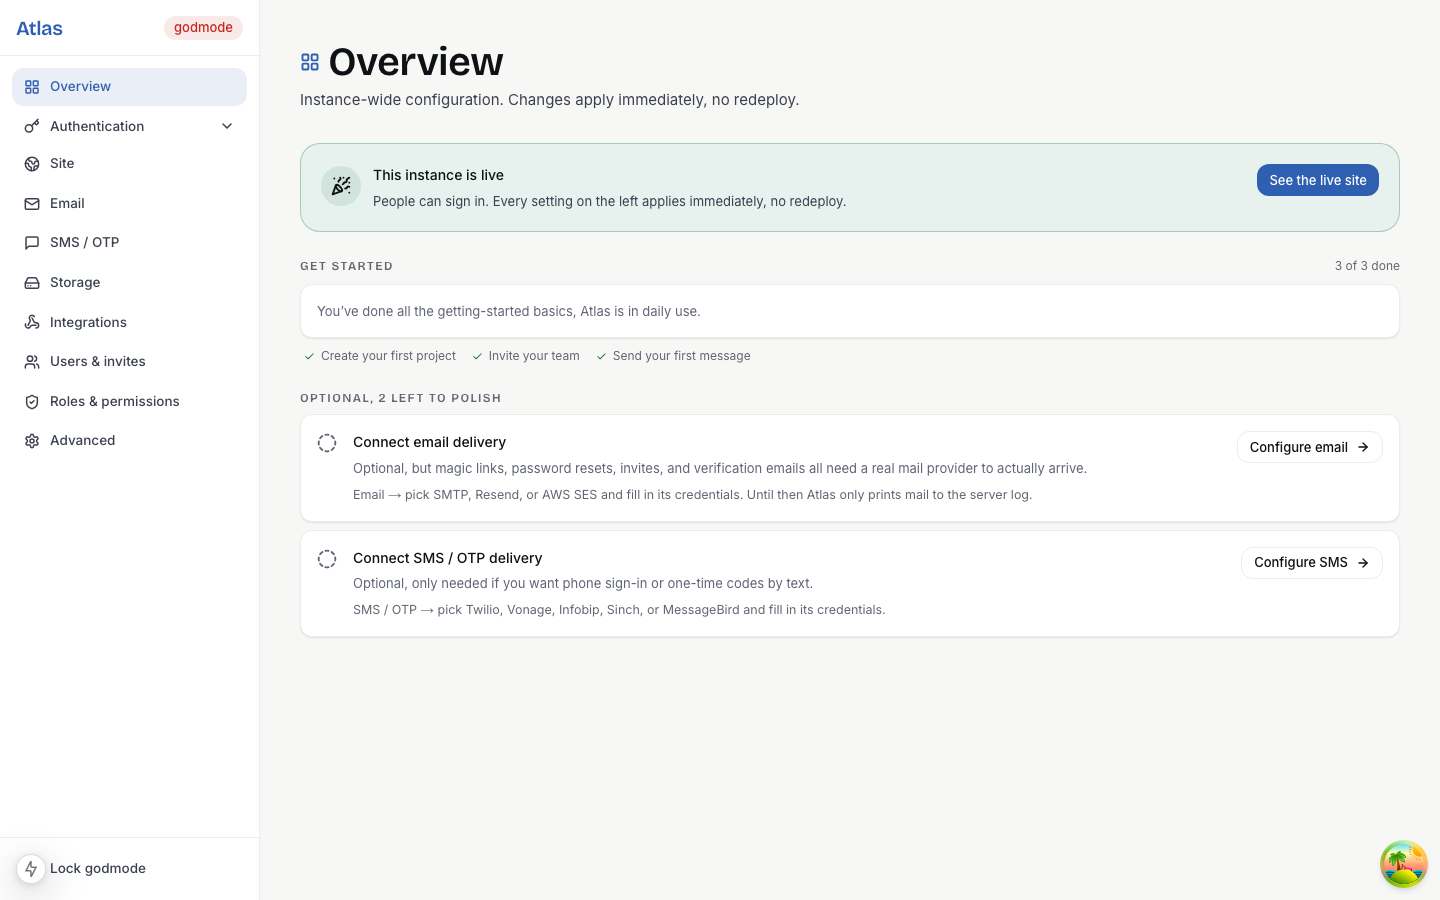
\includegraphics[width=0.485\linewidth]{assets/screenshots/curated/godmode-oauth.png}}
\caption{Godmode: ringkasan instans dan konfigurasi OAuth.}
\label{fig:godmode}
\end{figure*}

\subsection{24 Tema, Terang dan Gelap}

Setiap pengguna dapat memilih temanya sendiri dari 24 palet warna (masing-masing punya mode terang dan gelap), atau mengikuti tema bawaan yang ditetapkan admin. Seluruh tema melewati audit kontras WCAG otomatis sebelum bisa dirilis (\cref{fig:themes}).

\begin{figure*}[t]
\centering
\subfloat[Atlas Blue]{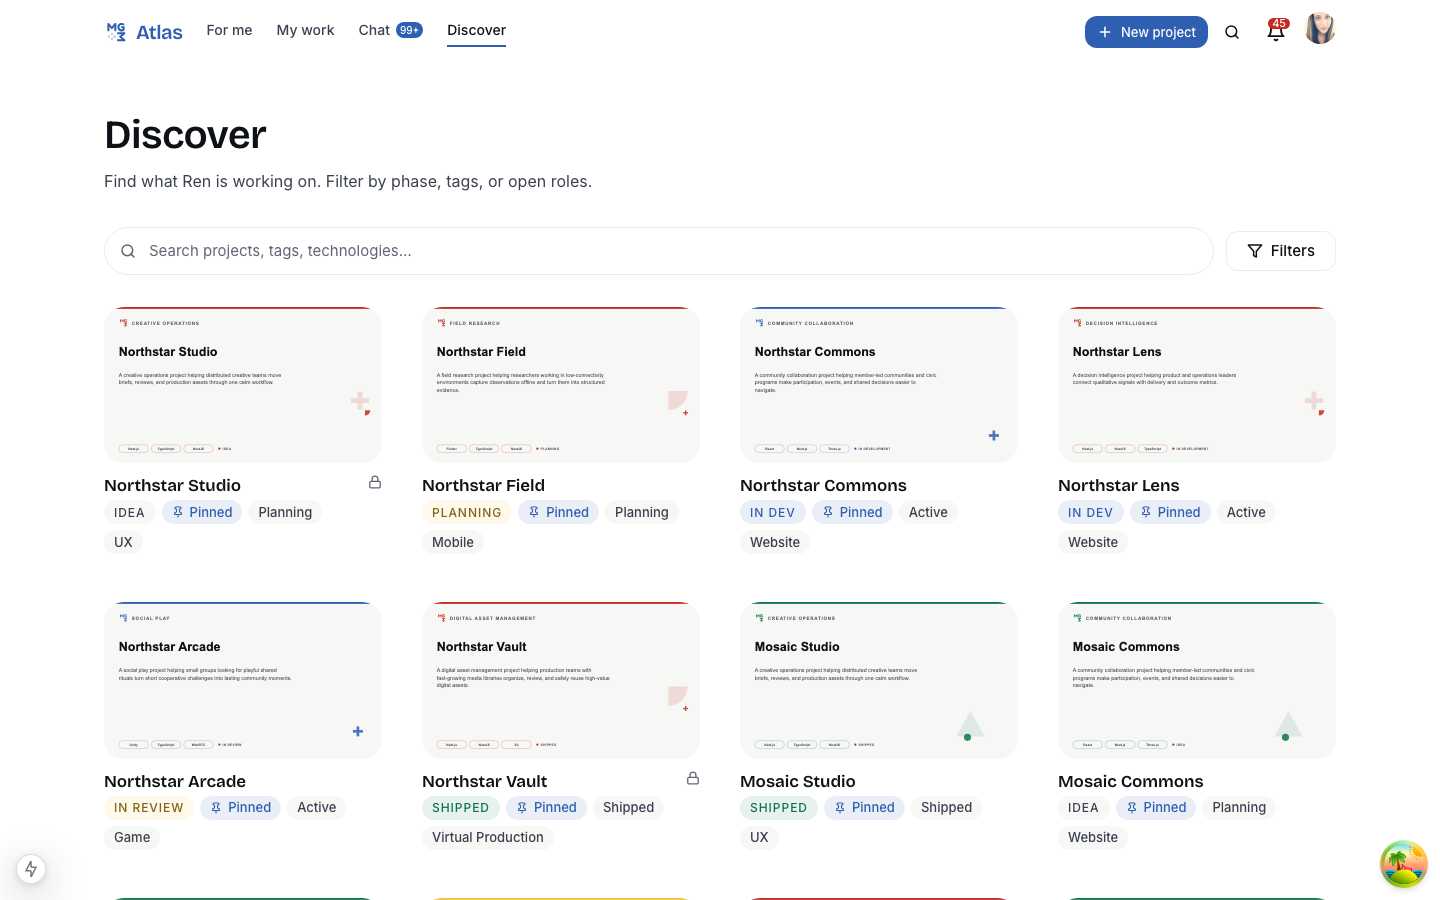
\includegraphics[width=0.24\linewidth]{assets/screenshots/curated/theme-atlas.png}}\hfill
\subfloat[Sunset]{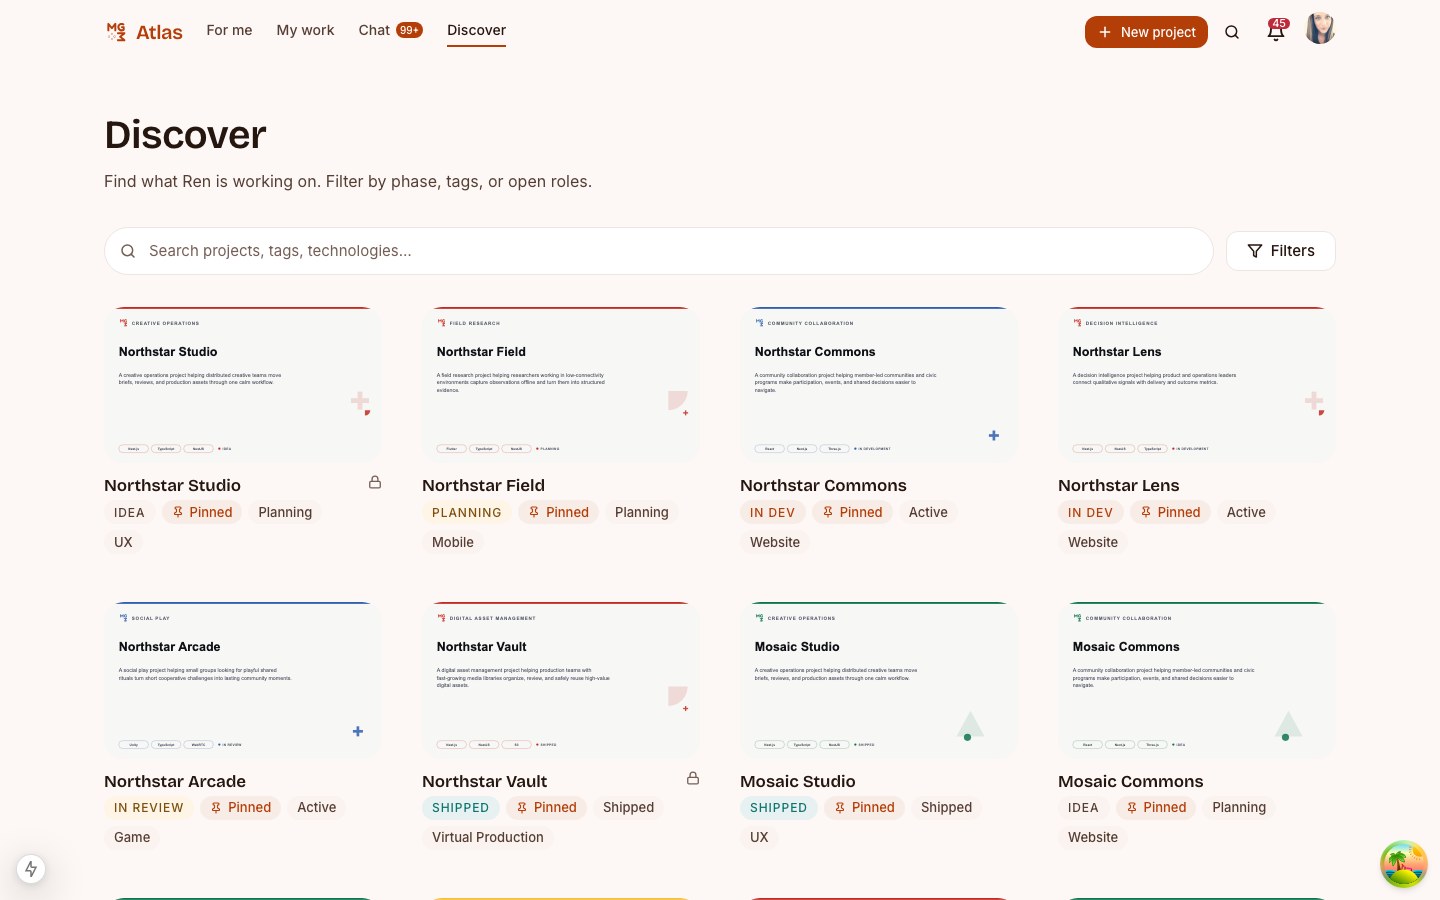
\includegraphics[width=0.24\linewidth]{assets/screenshots/curated/theme-sunset.png}}\hfill
\subfloat[Mint]{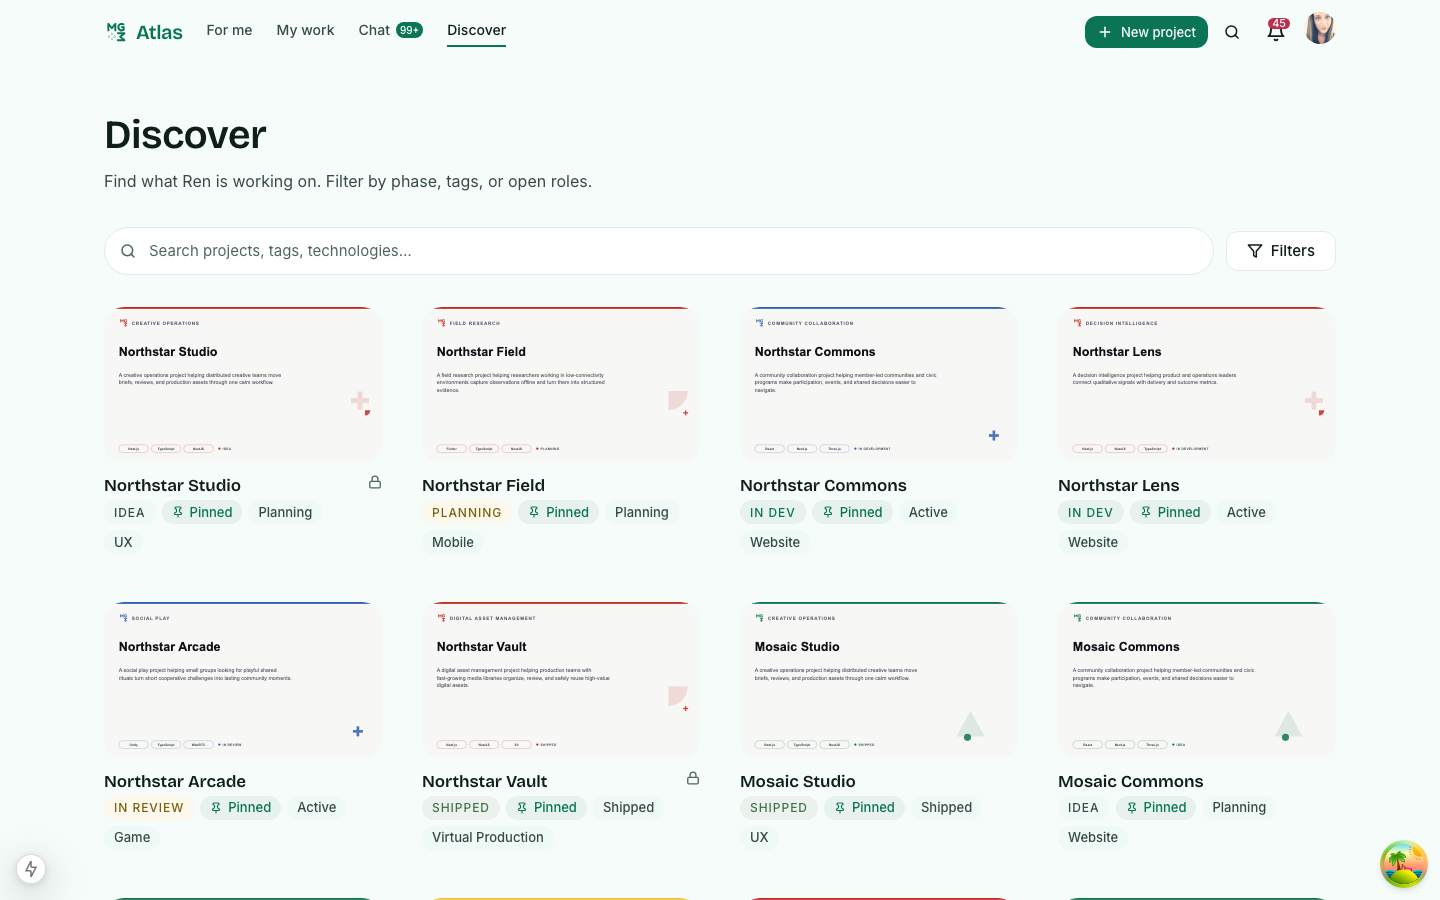
\includegraphics[width=0.24\linewidth]{assets/screenshots/curated/theme-mint.png}}\hfill
\subfloat[Lavender]{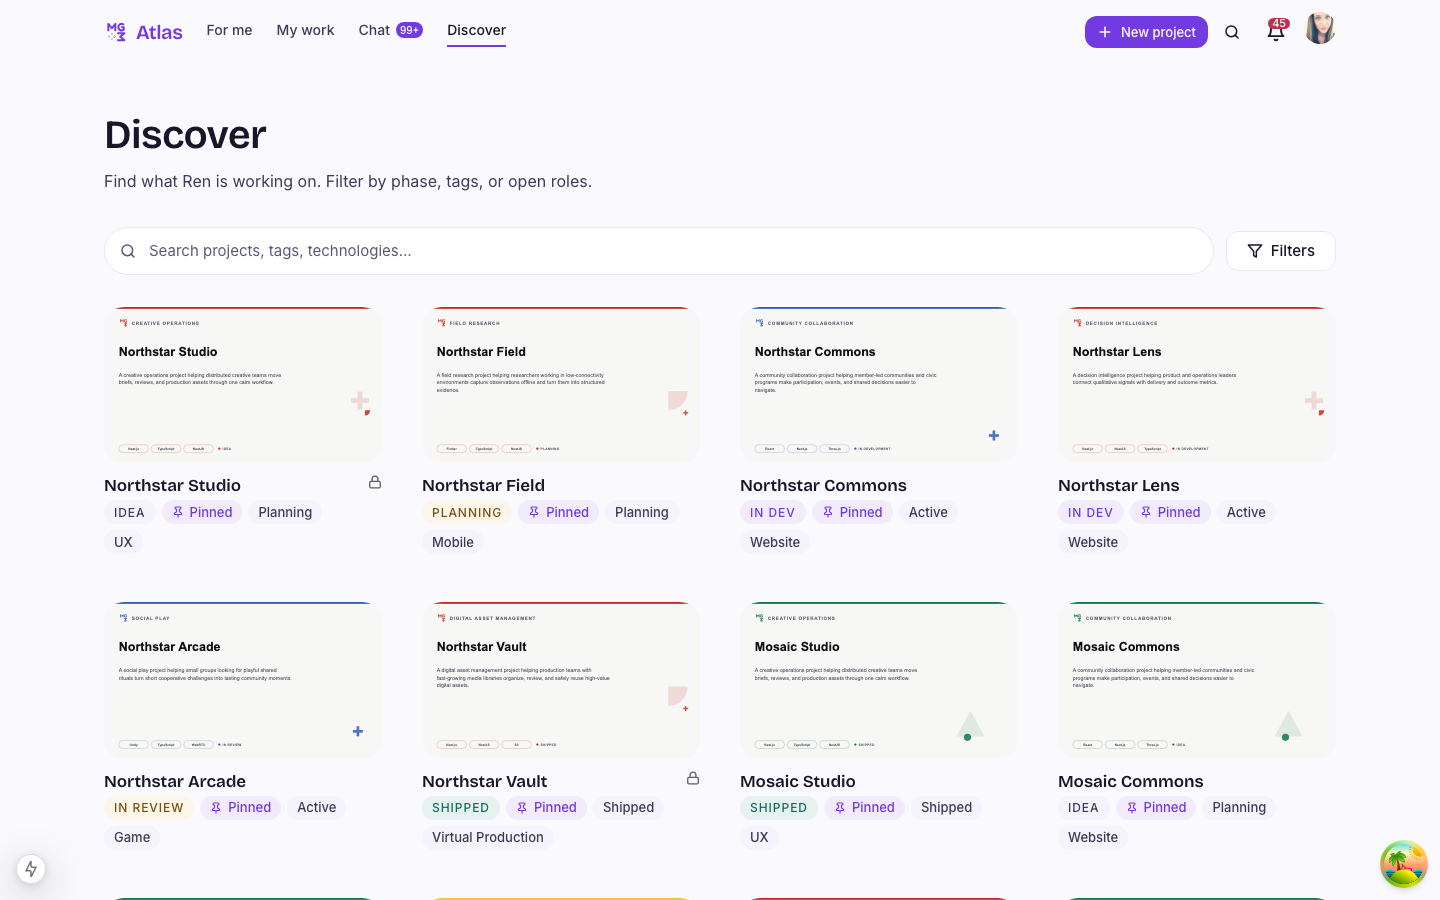
\includegraphics[width=0.24\linewidth]{assets/screenshots/curated/theme-lavender.png}}\\[4pt]
\subfloat[Deep Ocean]{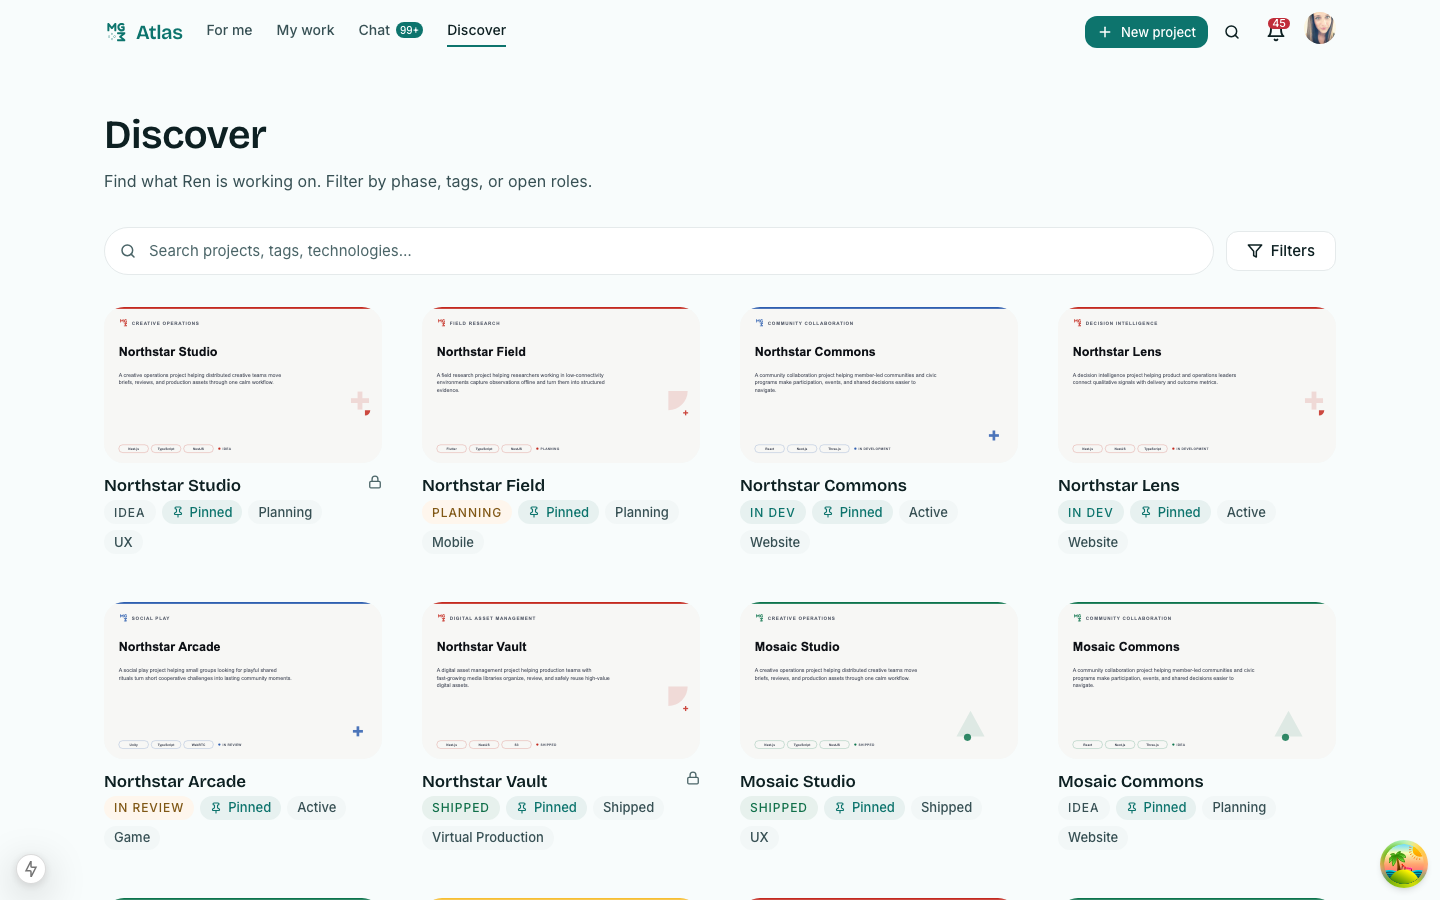
\includegraphics[width=0.24\linewidth]{assets/screenshots/curated/theme-ocean.png}}\hfill
\subfloat[Rose]{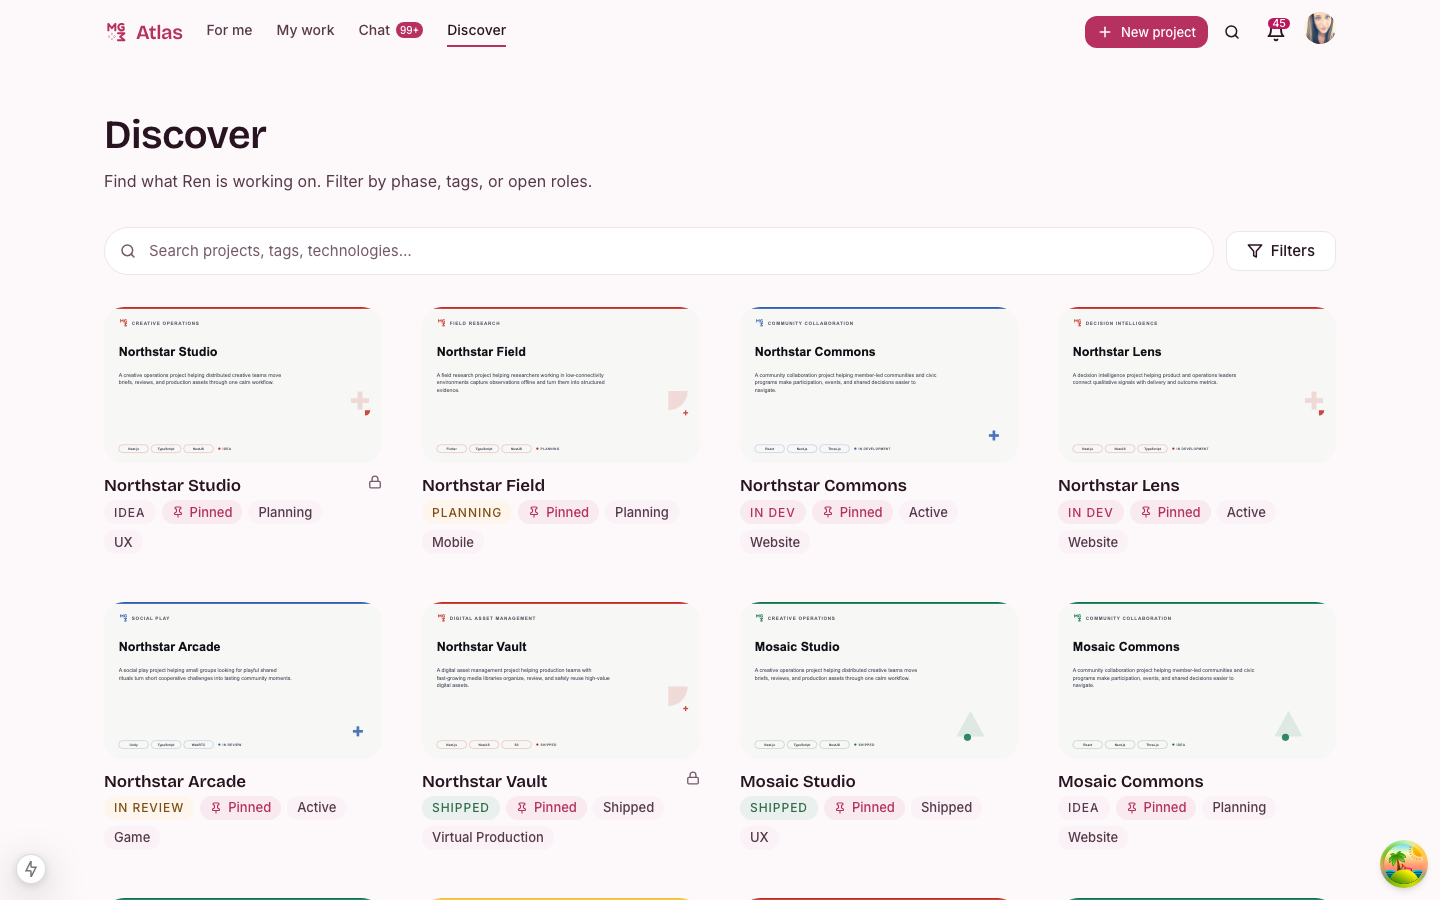
\includegraphics[width=0.24\linewidth]{assets/screenshots/curated/theme-rose.png}}\hfill
\subfloat[Midnight (gelap)]{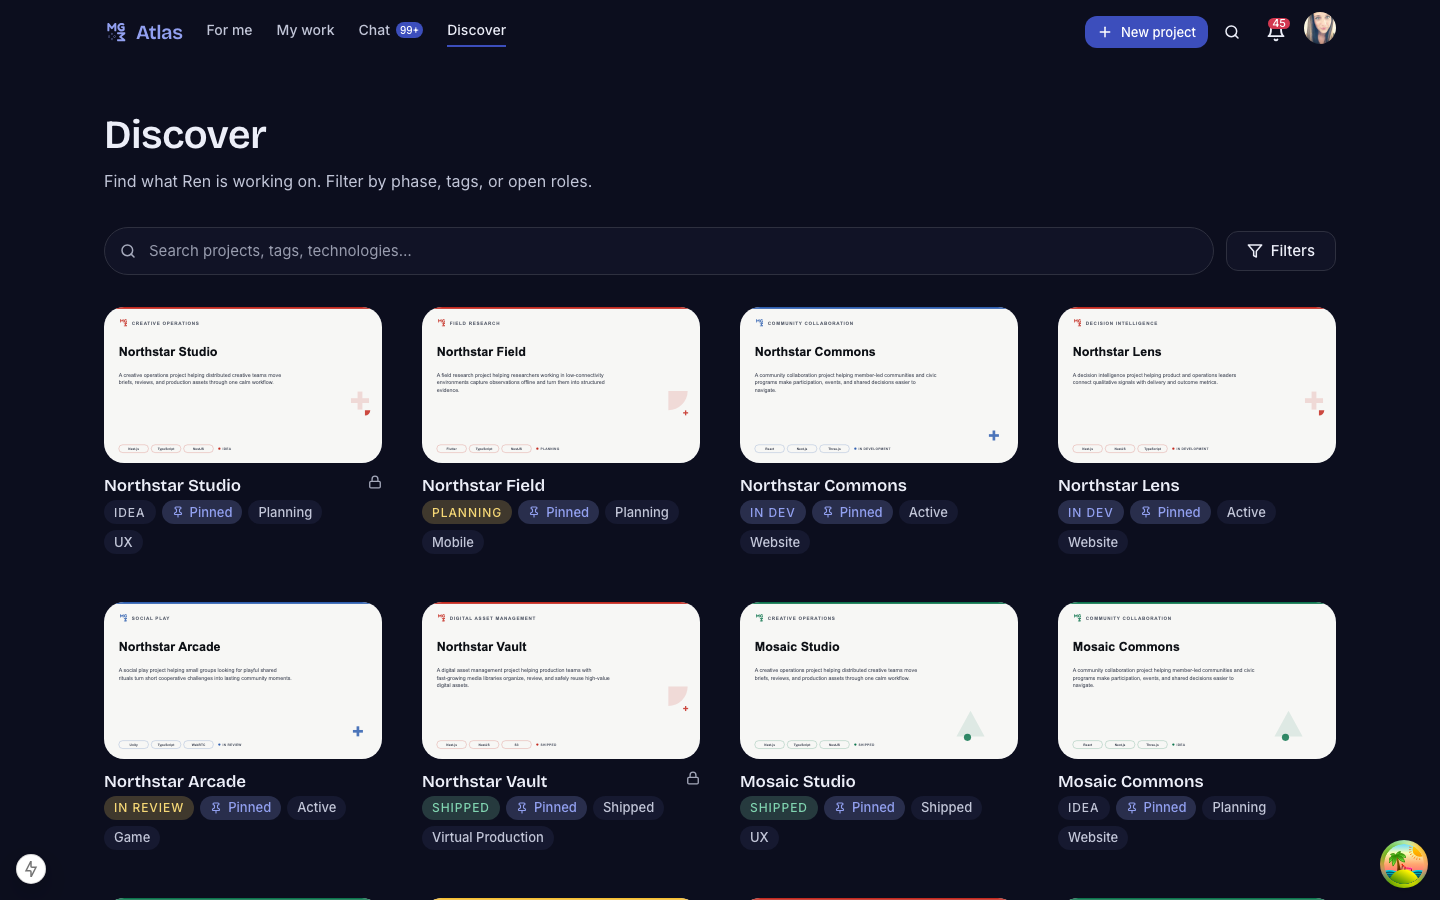
\includegraphics[width=0.24\linewidth]{assets/screenshots/curated/theme-midnight.png}}\hfill
\subfloat[Noir (gelap)]{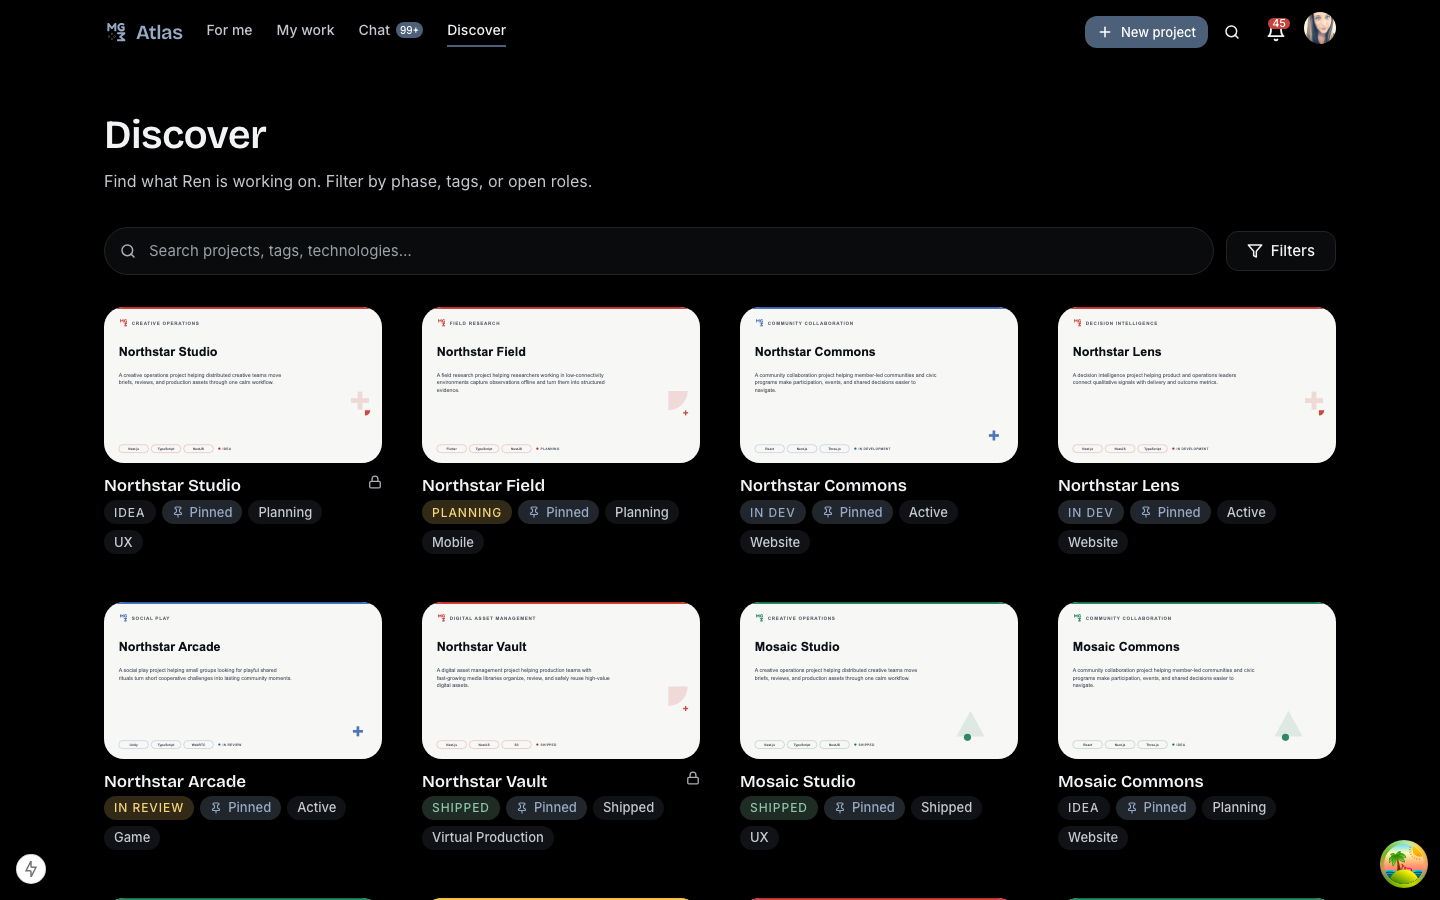
\includegraphics[width=0.24\linewidth]{assets/screenshots/curated/theme-noir.png}}
\caption{Delapan dari 24 tema yang tersedia, termasuk dua mode gelap.}
\label{fig:themes}
\end{figure*}

\subsection{Ringkasan modul lainnya}

\begin{description}
\item[Admin console.] Pengelolaan tag, peran kolaborasi, sticker, dan feature flag untuk operasional harian di luar Godmode.
\item[Catatan real-time.] Editor dokumen kolaboratif (BlockNote + Yjs) per daftar tugas, untuk brief, notulen, dan dokumentasi hidup.
\item[Notifikasi terpadu.] Satu pusat notifikasi untuk mention, penugasan tugas, dan pembaruan proyek, lintas seluruh modul.
\end{description}

\clearpage
\section[Metode Pengembangan]{}
\sectionopener{cyellow}{Cara Kerja Tim}{Metode Pengembangan}{Atlas dibangun dan terus disempurnakan lewat siklus iteratif pendek, ditarik langsung dari kebutuhan nyata pemakainya sendiri.}

\noindent
\begin{minipage}[t]{0.55\linewidth}
Karena tim pengembang adalah juga pengguna utama Atlas (anggota Laboratorium MGM), setiap siklus pengembangan dimulai dari gesekan nyata yang dialami sehari-hari, bukan asumsi di atas kertas. Pendekatan ini mendekati \textit{dogfooding} ala tim produk profesional: fitur diuji oleh pemakainya sendiri sebelum dianggap selesai.

\vspace{0.6em}
\begin{enumerate}[leftmargin=1.3em]
  \item \textbf{Temukan}: masalah diangkat dari keluhan atau kebutuhan nyata pengguna internal.
  \item \textbf{Rancang}: solusi diselaraskan dengan sistem desain MGM Laboratory yang sudah baku (token warna, tipografi, motif geometris).
  \item \textbf{Bangun}: implementasi di monorepo pnpm (frontend Next.js, backend NestJS), dengan tipe data yang disinkronkan lewat Prisma.
  \item \textbf{Uji}: audit otomatis (Jest untuk backend, Playwright + axe-core untuk audit UI lintas breakpoint dan aksesibilitas WCAG) sebelum rilis.
  \item \textbf{Rilis}: continuous deployment ke instans produksi yang sama yang dipakai laboratorium sehari-hari.
  \item \textbf{Pelajari}: masukan pemakai nyata langsung membentuk siklus berikutnya.
\end{enumerate}
\end{minipage}\hfill
\begin{minipage}[t]{0.4\linewidth}

\includegraphics[width=\linewidth]{assets/ai/opener-metode-pengembangan.png}
\end{minipage}

\vspace{1em}
\diagrambox{assets/diagrams/metode-cycle.pdf}{0.85}
\framecaption{Enam tahap yang berulang untuk setiap fitur baru maupun perbaikan.}

\subsection{Perkakas dan jaminan kualitas}

\noindent
\begin{minipage}[t]{0.31\linewidth}\featurecard{cyellow}{Monorepo terstruktur}{pnpm workspace dengan \texttt{apps/frontend} dan \texttt{apps/backend}, CI berbasis path filter agar hanya bagian yang berubah yang diuji ulang.}\end{minipage}\hfill
\begin{minipage}[t]{0.31\linewidth}\featurecard{cyellow}{Pengujian berlapis}{Jest untuk logika backend, Playwright untuk alur pengguna end-to-end, axe-core untuk audit aksesibilitas WCAG 2.1 AA otomatis.}\end{minipage}\hfill
\begin{minipage}[t]{0.31\linewidth}\featurecard{cyellow}{Migrasi basis data aditif}{Skema Prisma berkembang lewat migrasi yang selalu aditif, dijalankan otomatis (\texttt{migrate deploy}) setiap deployment produksi.}\end{minipage}

\clearpage

\section{Analisis Kebutuhan dan Desain}

Kebutuhan diturunkan langsung dari peran nyata yang setiap hari memakai Atlas di Laboratorium MGM.

\subsection{Tiga peran pengguna utama}

\begin{description}
\item[Admin instansi.] Mengatur metode masuk, integrasi, dan kebijakan seluruh instans lewat Godmode. Butuh kendali penuh tanpa harus membaca kode.
\item[Ketua proyek / koordinator.] Membagi pekerjaan lewat papan Kanban atau linimasa, memantau progres, dan menjaga proyek tidak macet di satu orang.
\item[Anggota / kontributor.] Perlu tahu tugas apa yang jadi tanggung jawabnya hari ini, dan bisa berkoordinasi tanpa berpindah aplikasi.
\end{description}

\subsection{Kebutuhan fungsional dan non-fungsional}

Tabel berikut merangkum kebutuhan lintas enam kategori, dari fungsional hingga portabilitas deployment.

\begin{table*}[t]
\centering
\caption{Kebutuhan fungsional dan non-fungsional Atlas.}
\label{tab:kebutuhan}
\small
\begin{tabular}{@{}L{3.2cm}L{13cm}@{}}
\toprule
\textbf{Kategori} & \textbf{Kebutuhan} \\
\midrule
Fungsional & Manajemen tugas multi-tampilan (Kanban/List/Timeline), obrolan real-time, panggilan suara, catatan \& whiteboard kolaboratif, notifikasi terpadu, manajemen peran dan izin \\
Otentikasi & Minimal enam metode masuk termasuk SSO institusi (SAML/OIDC), tanpa biaya tambahan pada jumlah pengguna berapa pun \\
Kinerja & Sinkronisasi dokumen dan suara real-time tidak melewati backend sebagai bottleneck (koneksi langsung peer-to-sidecar) \\
Keamanan & Sesi tervalidasi di basis data per permintaan, kata sandi di-\textit{hash} dengan bcrypt, rahasia godmode dienkripsi AES-256-GCM \\
Aksesibilitas & Kontras warna lolos audit WCAG otomatis di 24 tema $\times$ 2 mode, target sentuh minimal 36px \\
Portabilitas & Dapat di-\textit{deploy} lewat Docker Compose di infrastruktur mana pun, tidak terkunci pada satu penyedia cloud \\
\bottomrule
\end{tabular}
\end{table*}

\FloatBarrier
\subsection{Desain sebagai kebutuhan, bukan pemanis}

Sistem desain MGM Laboratory (token warna tertutup, tipografi Bricolage Grotesque + Geist, motif geometris satu warna per permukaan) diterapkan konsisten dari landing page hingga panel admin Atlas. Ini bukan keputusan kosmetik: produk yang dipakai 65+ orang setiap hari perlu terasa dapat dipercaya dan konsisten, sama seperti alasan tim akhirnya berhenti memakai kombinasi alat yang tampilannya saling bertabrakan.

\clearpage
\section[Arsitektur Sistem]{}
\sectionopener{cblue}{Di Bawah Tenda}{Arsitektur Sistem}{Semua ditulis dengan teknologi produksi yang matang, dipilih untuk keandalan jangka panjang, bukan sekadar demo kompetisi.}

\subsection{Tumpukan teknologi}

\begin{center}
\small
\renewcommand{\arraystretch}{1.35}
\begin{tabular}{@{}p{0.24\linewidth}p{0.72\linewidth}@{}}
\toprule
\tblhead{Lapisan} & \tblhead{Teknologi} \\
\midrule
Frontend & Next.js 15 (App Router), React 19, TypeScript, TanStack Query, Tailwind \\
Backend & NestJS 10, TypeScript, Prisma 5 ORM, class-validator \\
Basis data & PostgreSQL (dikelola Railway di produksi) \\
Cache \& rate limit & Redis \\
Real-time dokumen & Yjs (CRDT) lewat relay \texttt{y-websocket} khusus, untuk catatan dan whiteboard \\
Suara \& panggilan & LiveKit SFU (WebRTC) + LiveKit Egress untuk rekaman opsional \\
Penyimpanan berkas & Dapat dipilih lewat Godmode: disk lokal, S3, atau R2 (S3-compatible) \\
Otentikasi & Sesi opaque tersimpan di basis data, dikirim lewat header \texttt{Authorization: Bearer}, tanpa cookie maupun Auth.js/NextAuth \\
Lisensi & AGPL-3.0 (bersumber terbuka) \\
\bottomrule
\end{tabular}
\end{center}

\diagrambox{assets/diagrams/architecture.pdf}{1}
\framecaption{Backend menjadi jembatan kontrol; media suara dan sinkronisasi dokumen mengalir langsung antara browser dan sidecar-nya, tidak dibebankan ke backend.}

\clearpage
\subsection{Alur otentikasi}

Atlas tidak menggunakan Auth.js/NextAuth maupun cookie httpOnly. Setiap sesi adalah UUID acak (opaque) yang disimpan di basis data dan dikirim lewat header \texttt{Authorization: Bearer}, diverifikasi ulang di backend pada setiap permintaan lewat strategi \texttt{passport-custom}. Pendekatan ini mendukung enam metode masuk sekaligus: kata sandi, tautan ajaib, OTP telepon, kata sandi instans, OAuth2 (Google, GitHub, GitLab, Discord, dan lainnya), serta OIDC/SAML untuk direktori identitas institusi seperti Okta atau Entra ID, semuanya dikonfigurasi lewat Godmode tanpa deploy ulang.

\diagrambox{assets/diagrams/auth-flow.pdf}{0.92}

\vspace{1em}
\subsection{Topologi deployment}

Instans produksi Atlas (\texttt{atlas.creations.ren}) berjalan di Railway untuk layanan frontend, backend, dan basis data PostgreSQL terkelola, dengan LiveKit SFU dijalankan terpisah di VPS khusus (media WebRTC sebaiknya tidak berbagi jaringan dengan platform PaaS umum agar latensi suara tetap rendah), dan Cloudflare di depan untuk DNS.

\diagrambox{assets/diagrams/deployment.pdf}{0.92}

\clearpage
\subsection{Model data inti}

Skema Prisma lengkap mencakup lebih dari 40 tabel; berikut versi yang disederhanakan untuk menunjukkan relasi inti antara pengguna, proyek, tugas, dan komunikasi.

\diagrambox{assets/diagrams/erd.pdf}{1}

\clearpage

\section{Mockup / Gambaran Aplikasi}

Berbeda dari kebanyakan proposal kompetisi yang menyertakan \textit{wireframe} atau rancangan visual sebagai gambaran rencana, seluruh tangkapan layar Atlas dalam dokumen ini diambil dari aplikasi yang sudah dapat diakses dan digunakan sungguhan di \texttt{atlas.creations.ren}. Bagian ini memberikan gambaran tambahan yang belum ditunjukkan di bagian Fitur Aplikasi: halaman masuk, tampilan proyek, konsol admin, dan responsivitas di layar ponsel.

\begin{figure*}[t]
\centering
\subfloat[Halaman masuk menampilkan hanya metode otentikasi yang diaktifkan admin lewat Godmode.]{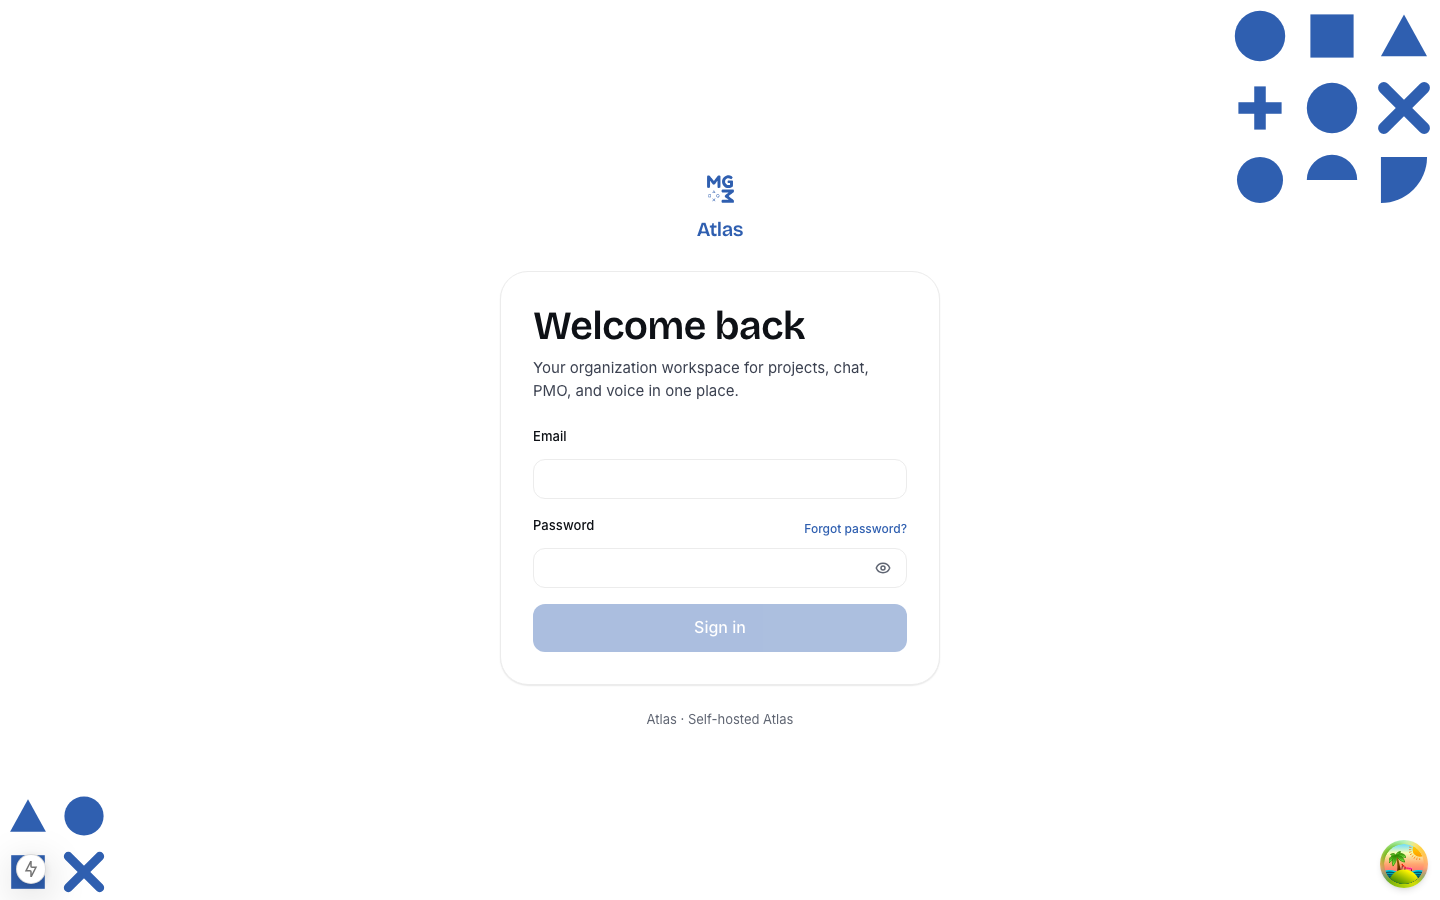
\includegraphics[width=0.485\linewidth]{assets/screenshots/curated/auth-login.png}}\hfill
\subfloat[Halaman ringkasan proyek, dengan sampul yang dibuat otomatis dari data proyek itu sendiri.]{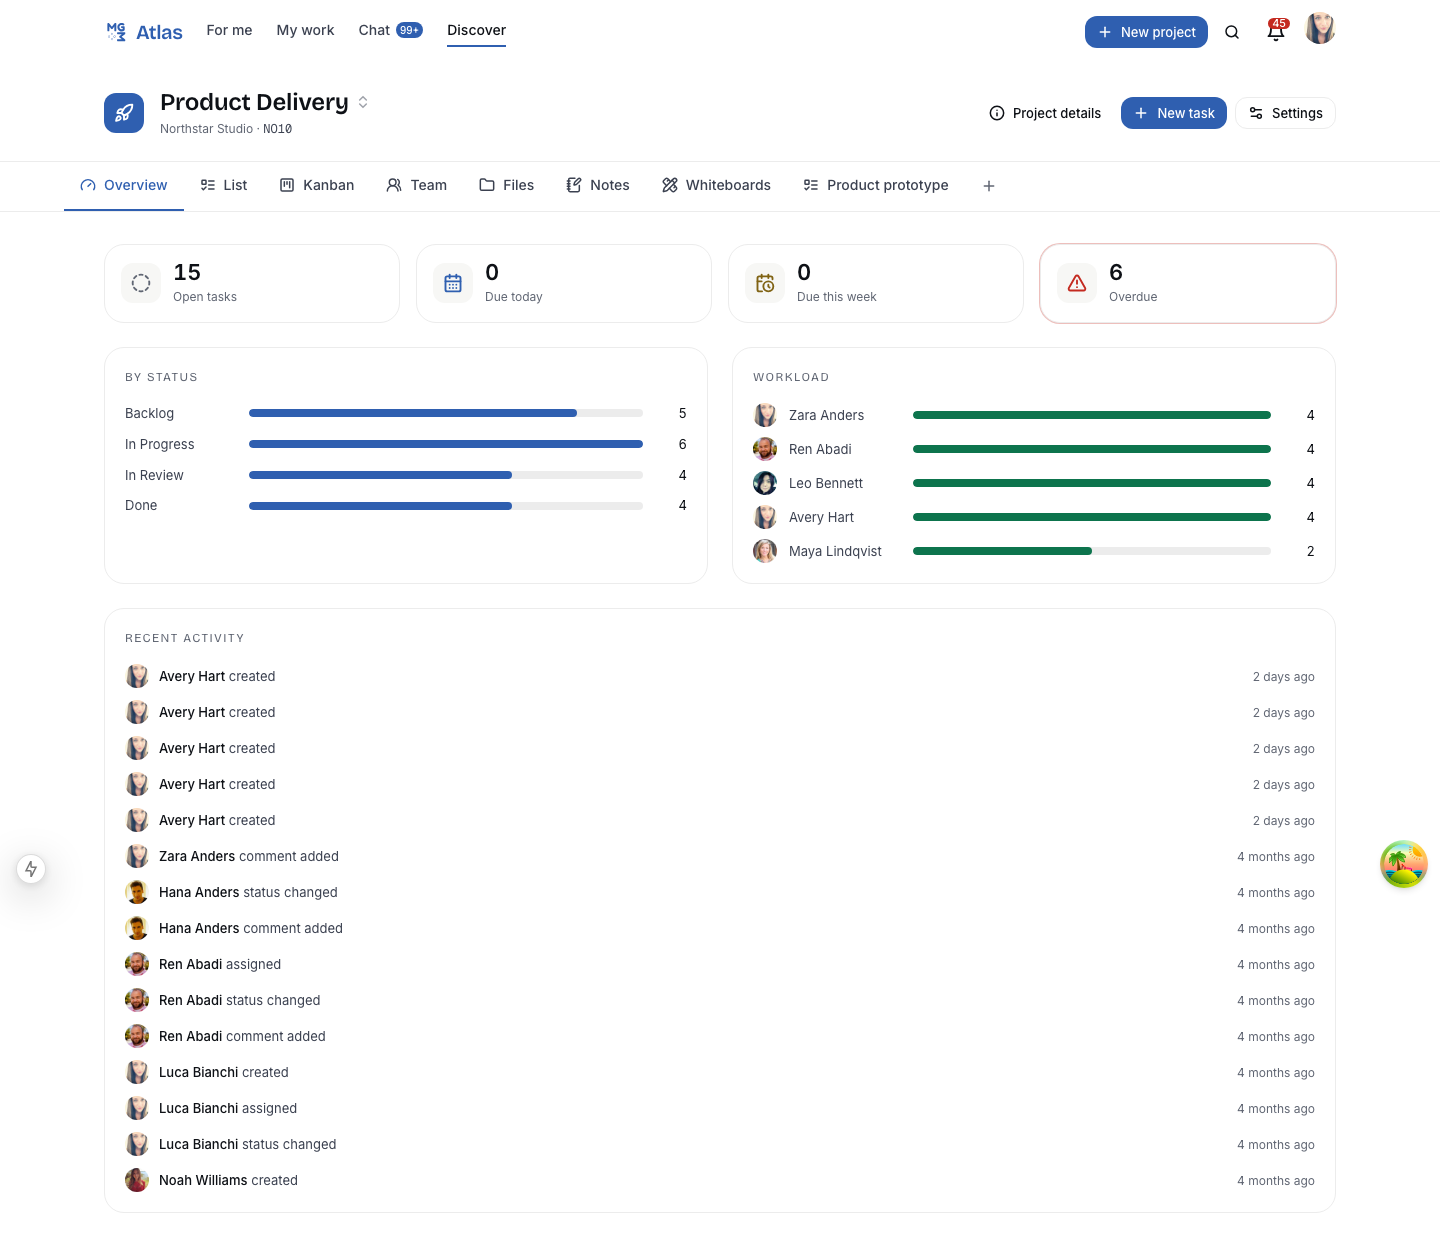
\includegraphics[width=0.485\linewidth]{assets/screenshots/curated/project-overview.png}}
\caption{Halaman masuk dan ringkasan proyek.}
\label{fig:mockup-login-project}
\end{figure*}

\FloatBarrier
\begin{figure*}[t]
\centering
\subfloat[Konsol admin: pengelolaan pengguna di luar panel Godmode.]{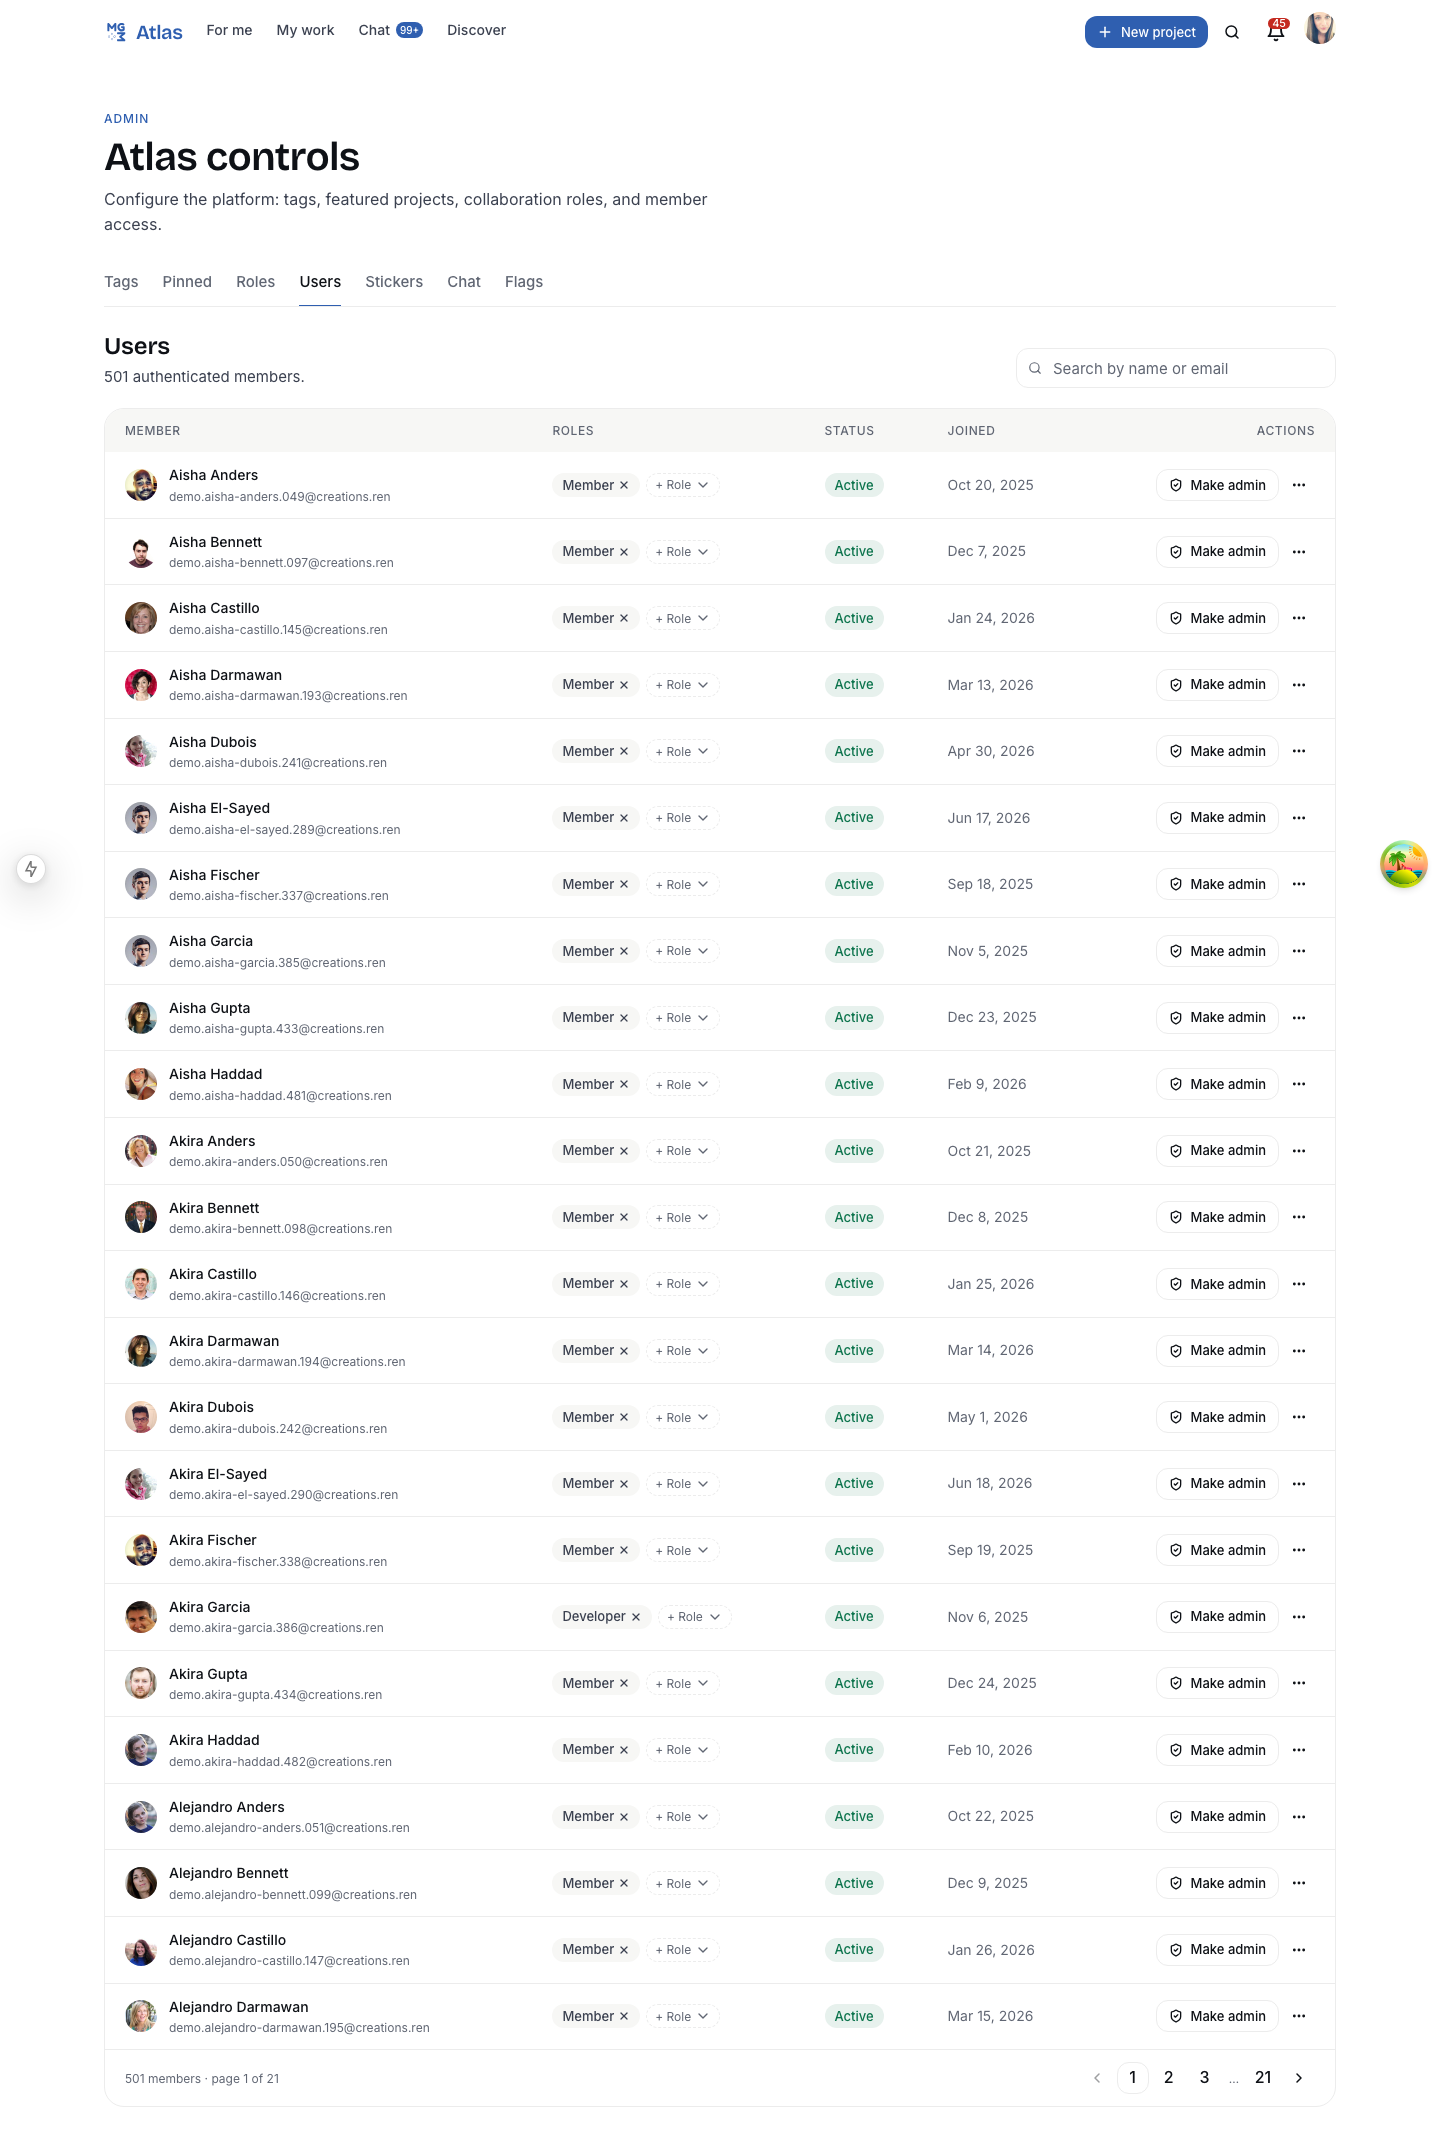
\includegraphics[width=0.485\linewidth]{assets/screenshots/curated/admin-users.png}}\hfill
\subfloat[Konfigurasi SSO institusi (OIDC/SAML) tanpa biaya tambahan.]{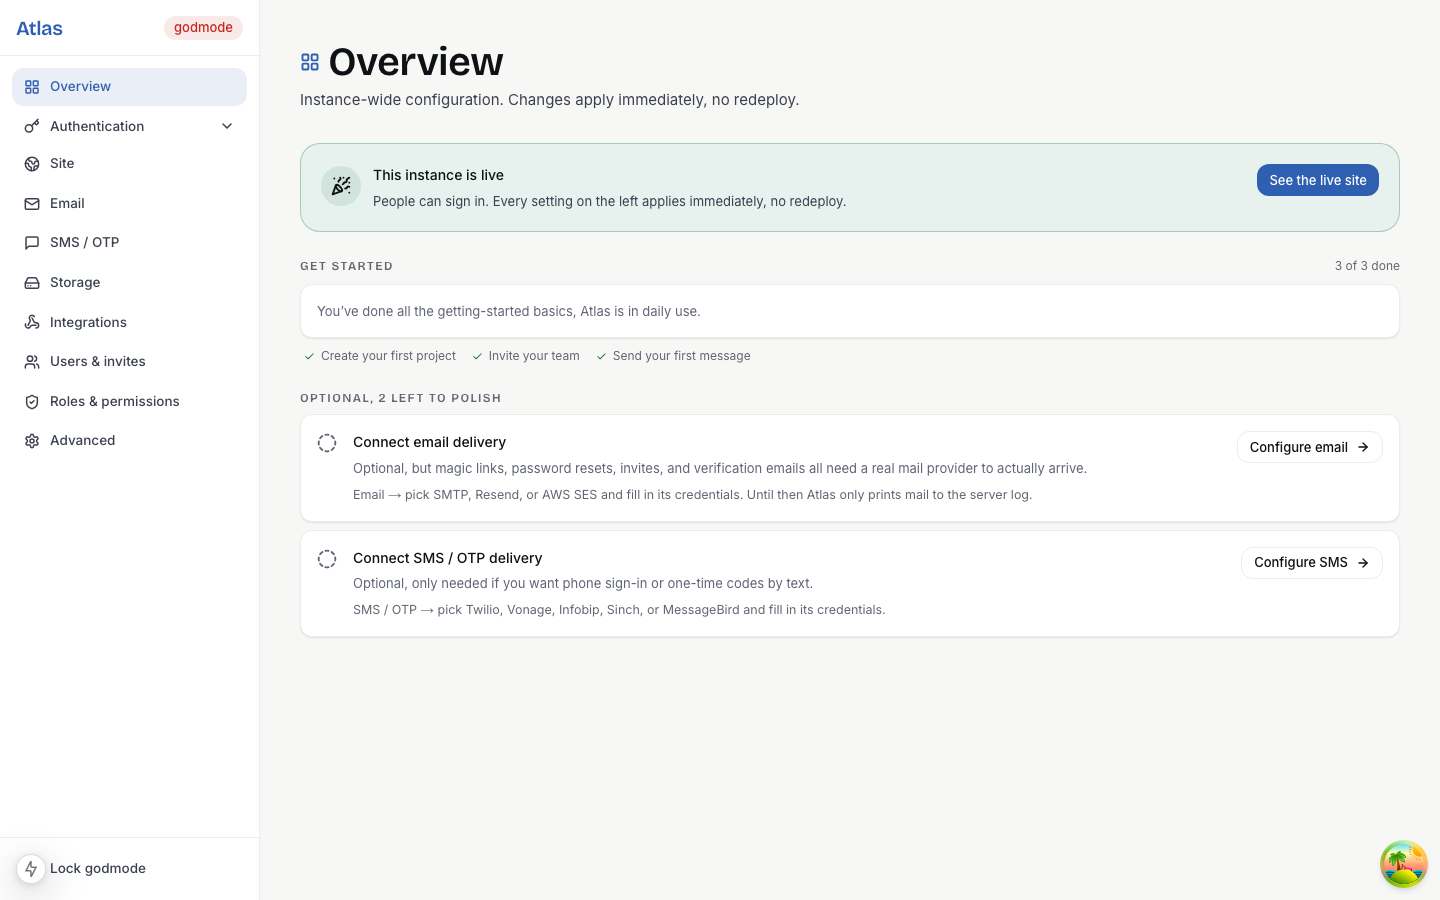
\includegraphics[width=0.485\linewidth]{assets/screenshots/curated/godmode-sso.png}}
\caption{Konsol admin dan konfigurasi SSO.}
\label{fig:mockup-admin-sso}
\end{figure*}

\FloatBarrier
\subsection{Responsif di layar ponsel}

Seluruh antarmuka melewati audit responsif lintas breakpoint (360 hingga 1920px), termasuk navigasi yang berubah jadi \textit{drawer} pada layar sempit dan target sentuh minimal 36px.

\begin{figure*}[t]
\centering
\subfloat[Discover]{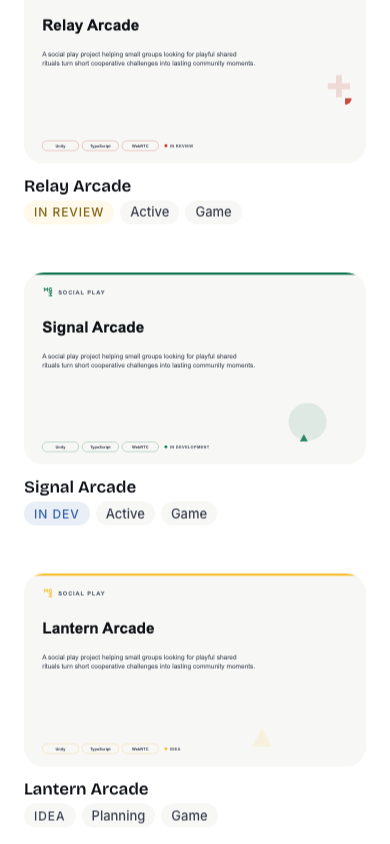
\includegraphics[width=0.31\linewidth]{assets/screenshots/curated/mobile-dashboard.png}}\hfill
\subfloat[Kanban]{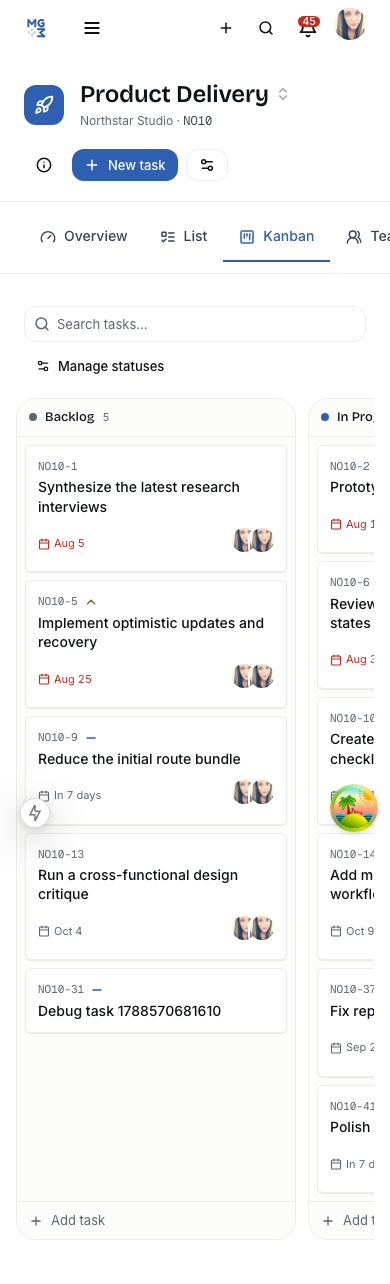
\includegraphics[width=0.31\linewidth]{assets/screenshots/curated/mobile-kanban.png}}\hfill
\subfloat[Chat]{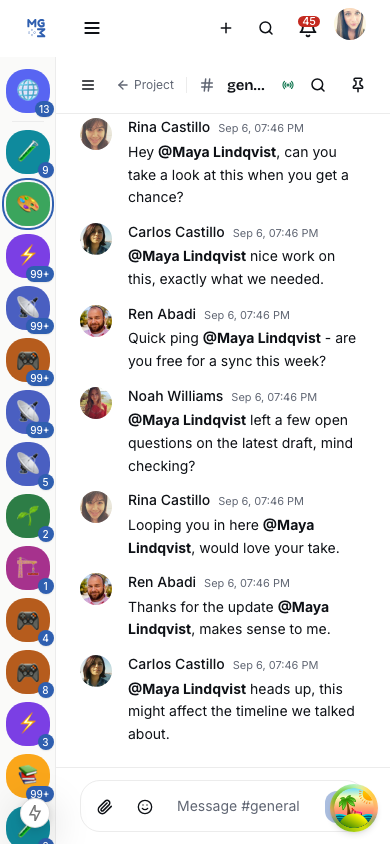
\includegraphics[width=0.31\linewidth]{assets/screenshots/curated/mobile-chat.png}}
\caption{Tiga tampilan Atlas di viewport ponsel (390px).}
\label{fig:mobile}
\end{figure*}

\FloatBarrier

\clearpage
\section[Rencana Implementasi]{}
\sectionopener{cgreen}{Peta Jalan}{Rencana Implementasi}{Atlas tidak dimulai dari nol pasca-kompetisi: pondasi produksi sudah berjalan, rencana ke depan adalah memperluas jangkauan dan memperkuat keandalannya.}

\diagrambox{assets/diagrams/roadmap.pdf}{1}

\vspace{1em}
\subsection{Rincian setiap tahap}

\begin{enumerate}[leftmargin=1.4em]
  \item \textbf{Sekarang, MVP produksi.} Seluruh modul (PMO, chat, suara, catatan/whiteboard real-time, Godmode) berjalan dan dipakai harian oleh Laboratorium MGM; bersumber terbuka di bawah AGPL-3.0.
  \item \textbf{Jangka pendek.} Perluasan pengujian bersama komunitas dan himpunan kampus lain, penguatan audit keamanan (terutama alur otentikasi multi-metode), serta perbaikan berdasarkan umpan balik pemakai nyata di luar MGM Laboratory.
  \item \textbf{Menengah.} Aplikasi mobile pendamping, integrasi kalender dan email eksternal, serta ekspor/impor data untuk migrasi dari alat lain (Jira, Trello, Notion).
  \item \textbf{Panjang.} Sistem plugin/integrasi pihak ketiga, dan dukungan federasi multi-instans agar organisasi besar dapat menghubungkan beberapa deployment Atlas tanpa kehilangan kendali data masing-masing.
\end{enumerate}

\vspace{0.6em}
\begin{calloutbox}{cgreen}
{\bricolagesb\fontsize{11pt}{14pt}\selectfont\color{cink} Mengapa peta jalan ini realistis}\\[0.3em]
{\fontsize{9.6pt}{13pt}\selectfont\color{cink2} Setiap tahap dibangun di atas kode yang sudah berjalan produksi, bukan proposal fitur yang belum tersentuh. Tim tidak perlu meyakinkan pemakai baru bahwa Atlas ``akan'' berfungsi, sebab 65+ pemakai nyata sudah membuktikannya setiap hari.}
\end{calloutbox}

\clearpage

\clearpage
\section[Lampiran]{}
\sectionopener{cred}{Penutup}{Lampiran}{Tautan, kredensial uji coba, dan pernyataan orisinalitas tim.}

\subsection{Akses dan tautan}

\begin{center}
\small
\renewcommand{\arraystretch}{1.4}
\begin{tabular}{@{}p{0.28\linewidth}p{0.68\linewidth}@{}}
\toprule
\tblhead{Item} & \tblhead{Tautan / Keterangan} \\
\midrule
Aplikasi produksi & \url{https://atlas.creations.ren} \\
Akun demo untuk juri & Disediakan pada bundel pengumpulan (Google Drive) bersama README, agar akun uji coba tidak tercampur dengan data operasional nyata Laboratorium MGM yang berjalan di instans yang sama \\
Kode sumber & Berkas \texttt{.zip} pada bundel pengumpulan, disertai \texttt{README.md} berisi panduan instalasi, spesifikasi lingkungan, dan cara menjalankan secara lokal \\
Video demo & Tautan YouTube/Google Drive dicantumkan pada bundel pengumpulan \\
Lisensi & AGPL-3.0 (bersumber terbuka, dapat dimodifikasi dan di-\textit{deploy} ulang secara bebas) \\
\bottomrule
\end{tabular}
\end{center}

\vspace{0.8em}
\subsection{Tim MGM Unjuk Diri Dulu}

\noindent
\begin{minipage}[t]{0.31\linewidth}
\eyebrow{cred}{Ketua Tim}\\[0.3em]
{\fontsize{10.5pt}{15pt}\selectfont\bricolagesb\color{cink} Muhammad Idham Ma'arif}\\
{\fontsize{9pt}{13pt}\selectfont\color{cink3} NIM 245150300111024}\\
{\fontsize{9pt}{13pt}\selectfont\color{cink3} Universitas Brawijaya}
\end{minipage}\hfill
\begin{minipage}[t]{0.31\linewidth}
\eyebrow{cred}{Anggota}\\[0.3em]
{\fontsize{10.5pt}{15pt}\selectfont\bricolagesb\color{cink} Syafa Hadyan Rasendriya}\\
{\fontsize{9pt}{13pt}\selectfont\color{cink3} Universitas Brawijaya}
\end{minipage}\hfill
\begin{minipage}[t]{0.31\linewidth}
\eyebrow{cred}{Anggota}\\[0.3em]
{\fontsize{10.5pt}{15pt}\selectfont\bricolagesb\color{cink} Nurul Inayah}\\
{\fontsize{9pt}{13pt}\selectfont\color{cink3} Universitas Brawijaya}
\end{minipage}

\vspace{1.2em}
\subsection{Pernyataan orisinalitas}

\begin{calloutbox}{cred}
{\fontsize{9.6pt}{14pt}\selectfont\color{cink2}
Tim menyatakan bahwa Atlas merupakan karya asli yang dikembangkan sendiri, belum pernah dipublikasikan atau memenangkan kompetisi sejenis sebelumnya, dan tidak melanggar hak kekayaan intelektual pihak lain. Surat pernyataan orisinalitas yang telah ditandatangani seluruh anggota tim, menggunakan templat resmi panitia HOLOGY 9.0, dilampirkan sebagai berkas terpisah pada bundel pengumpulan.
}
\end{calloutbox}

\vspace{1.5em}
\begin{center}
{\geistmono\fontsize{8pt}{11pt}\selectfont\color{cink4} ATLAS \textbullet\ HOLOGY 9.0 HOLODEV \textbullet\ MGM UNJUK DIRI DULU \textbullet\ UNIVERSITAS BRAWIJAYA \textbullet\ 2026}
\end{center}


\end{document}
